% !TeX root = RJwrapper.tex
\title{bayesanova: An R package for Bayesian Inference in the Analysis of Variance via Markov Chain Monte Carlo in Gaussian Mixture Models}
\author{by Riko Kelter}

\maketitle

\abstract{
This paper introduces the R package \CRANpkg{bayesanova}, which performs Bayesian inference in the analysis of variance (ANOVA). Traditional ANOVA based on null hypothesis significance testing (NHST) is prone to overestimating effects and stating effects if none are present. Bayesian ANOVAs developed so far are based on Bayes factors (BF), which also enforce a hypothesis testing stance. Instead, the Bayesian ANOVA implemented in \pkg{bayesanova} focusses on effect size estimation and is based on a Gaussian mixture with known allocations, for which full posterior inference for the component parameters is implemented via Markov-Chain-Monte-Carlo (MCMC). Inference for the difference in means, standard deviations and effect sizes between each of the groups is obtained automatically. Estimation of the parameters instead of hypothesis testing is embraced via the region of practical equivalence (ROPE), and helper functions provide checks of the model assumptions and visualization of the results.
}


\section[Introduction]{Introduction} \label{sec:intro}

%\begin{leftbar}
This article introduces \CRANpkg{bayesanova}, an R package for conducting a Bayesian analysis of variance (ANOVA) via Markov Chain Monte Carlo (MCMC) in a Gaussian mixture model. Classic frequentist analysis of variance is based on null hypothesis significance testing (NHST), which recently has been shown to produce serious problems regarding the reproducibility and reliability of scientific results \citep{benjaminRedefineStatisticalSignificance, Colquhoun2017, Colquhoun2019, Wasserstein2019, wasserstein2016}. NHST is based on test statistics, $p$-values and significance levels $\alpha$, which are designed to control the long-term false-positive rate. Still, in a multitude of settings these approaches do in fact lead to an inflated rate of false-positive results, undermining the validity and progress of science. Examples include optional stopping of participant recruiting in studies \citep{Carlin2009} or the necessary testing for violations of distributional assumptions which some frequentist hypothesis tests make \citep{Rochon2012}. 

As a solution to these problems, Bayesian methods have been proposed recently and are since gaining popularity in a wide range of scientific domains \citep{McElreath2015, Kruschke2013, Kruschke2015}. The Bayesian philosophy proceeds by combining the model likelihood $f(x|\theta)$ with the available prior information $p(\theta)$ to obtain the posterior distribution $f(\theta|x)$ through the use of Bayes' theorem:
\begin{equation} \label{eq:mean}
f(\theta|x) \propto f(x|\theta) f(\theta)
\end{equation}
While the Bayesian philosophy thus allows for flexible modeling, inference for the posterior distribution $f(\theta|x)$ can be complicated in practice. Therefore, Markov chain Monte Carlo techniques have been developed, which make use of the facts that (1) constructing a Markov chain which has the posterior distribution $f(\theta|x)$ as its stationary distribution, and (2) drawing samples from this Markov chain to approximate the posterior $f(\theta|x)$ can be used to obtain the posterior numerically.

The \pkg{bayesanova} package is designed as a Bayesian alternative to the frequentist analysis of variance. By using a Gaussian mixture model and implementing a Markov Chain Monte Carlo algorithm for this model, full posterior inference can be obtained. This allows for explicit hypothesis testing between groups as in the frequentist ANOVA, or for estimation of parameters under uncertainty. The focus in \pkg{bayesanova} is on the latter perspective and avoids explicit hypothesis testing. While Bayesian versions of the analysis of variance have been proposed recently by \cite{Rouder2012} and \cite{Bergh2019ANOVAJasp}, these implementations focus on the Bayes factor as a measure of evidence \citep{VanDoorn2019, Jasp2019}. As the Bayes factor suffers from multiple problems, one of which is its strong dependence on the used priors -- see \cite{Kamary2014} and \cite{Robert2016} -- the implementation in \pkg{bayesanova} avoids the Bayes factor and uses a different posterior index, the region of practical equivalence (ROPE) \citep{Kruschke2018a}, which has lately been shown to have some desirable properties, in particular in contrast to the Bayes factor \citep{Makowski2019}. 

The plan of the paper is as follows: The next section introduces the analysis of variance in a frequentist and Bayesian fashion and gives an overview about packages implementing these methods. The following section then introduces the novel approach implemented in \pkg{bayesanova}. The details on the mixture representation of the Bayesian analysis of variance are discussed and scenarios where \pkg{bayesanova} is designed to be used are detailed. The section thereafter outlines the structure of the package and details the included functions. The following section presents a variety of examples and illustrations using real datasets from biomedical and psychological research as well as synthetic datasets. The last section then provides a summary of the benefits and drawbacks of the used implementation, as well as future plans for the package.


\section{Frequentist and Bayesian analysis of variance} \label{sec:anova}
\subsection{Traditional ANOVA models using NHST via the F-statistic}
In applied statistics, the one-way analysis of variance is a method which can be used to compare means of two or more samples (typically three). The one-way ANOVA assumes numerical (response) data in each group and (usually) categorical input data like a group indicator in a randomized clinical trial (RCT). Interpreting the ANOVA as a linear model, one obtains for data $y_{i,j}$, where $i=1,...,n$ is an index over the experimental units (patients, participants) and $j=1,...,k$ an index over treatment groups
\begin{equation} \label{eq:mean}
y_{i,j}=\mu_j+\varepsilon_{i,j}
\end{equation}
if the experiment is completely randomized. Here, $\varepsilon \sim \mathcal{N}(0,\sigma^2)$ so that $\varepsilon_{i,j}$ are normally distributed zero-mean residuals. $\mu_j$ is the mean of treatment group $j$ and $y_{i,j}$ the response variable which is measured in the experiment.

The one-way ANOVA then tests the null hypothesis $H_0$ that all samples are drawn from populations with identical means. To do this, (1) two estimates of the population variance are obtained which rely on various assumptions and (2) an F-statistic is produced by the ANOVA, which is the ratio of variance calculated among the means to the variance within the samples. The intuition here is that if group means are drawn from populations with identical means, the variance of the group means should be smaller than the variance of samples and a high ratio thereby indicates differing means. Mathematical details on computing the F-statistic can be found in the Appendix.

The one-way ANOVA as detailed above makes several assumptions, the most important of which are: (1) variances of populations are equal; (2) responses for a given group are independent and identical distributed random variables; (3) response variable residuals are normally distributed, that is $\varepsilon \sim \mathcal{N}(0,\sigma^2)$.

While Monte Carlo studies have shown that the ANOVA is quite robust to small to medium violations of these assumptions \citep{Donaldson1966}, severe violations of assumptions (1)-(3) will result in inflated rates of false positives and and thereby unreliable results \citep{Tiku1971}.

\subsection{Bayesian ANOVA models}
Bayesian models for the ANOVA have been developed recently to solve some of the problems of NHST. The developed models can be categorized broadly into two approaches: The first approach relies on the Bayes factor as a measure of relative evidence and was developed by \cite{Rouder2012}. The second approach is based on MCMC algorithms like Gibbs sampling in JAGS \citep{Plummer2003} or Hamiltonian Monte Carlo (HMC) in Stan \citep{Carpenter2017, RStan2020}. This approach was popularized by \cite{Kruschke2015}. Here the region of practical equivalence (ROPE) as introduced by \cite{Kruschke2015} is used for measuring the evidence given the data. Also, an explicit hypothesis testing stance is avoided.



%They start with the one-sample model, where $y_{i}\sim \mathcal{N}(\mu,\sigma^2)$ for $i=1,...,n$ i.i.d., so there is just a single population. The research question thus reduces to whether the mean of that population is zero, $\mu=0$. Following \cite{jeffreys1961} by reparameterizing $\delta=\mu/\sigma$, where $\delta$ is the effect size of \cite{cohen_statistical_1988}, the model can be rewritten as
%\begin{align}
%	y_i \sim \mathcal{N}(\sigma \delta,\sigma^2)	
%\end{align}
%and the null and alternative model to compare differ only in the choice of priors on $\delta$:
%\begin{align}
%	\mathcal{M}_0:\delta=0 \hspace{1cm} \mathcal{M}_1:\delta \sim \text{Cauchy}	
%\end{align}
%Putting a Jeffreys prior on the only remaining model parameter $\sigma^2$, $p(\sigma^2)\propto 1/\sigma^2$, the Bayes factor $BF_{01}$ can be calculated as the one-dimensional integral
%\begin{align}
%	BF_{01}(t,N)=\frac{(1+\frac{t^2}{N-1})^{-N/2}}{\int_0^\infty (1+Ng)^{-1/2} (1+\frac{t^2}{(1+Ng)(N-1)})^{-N/2}p(g)dg}	
%\end{align}
%where $p(g)=(2\pi)^{-1/2}g^{-3/2}e^{-1/(2g)}$ and $t=\bar{y}\sqrt{N}/s_y$ is the t-statistic observed with $\bar{y}$ and $s_y$ the sample mean and standard deviation and $N$ the sample size. For details and a proof see the appendix in \cite{Rouder2012}.

%This one-sample design is based on \cite{Rouder2009} and extended by \cite{Rouder2012} to the multivariate case. 
The approach of \cite{Rouder2012} can be summarized as follows:  An independent Cauchy prior is considered
\begin{align}\label{eq:indepCauchyPrior}
	p(\theta)=\prod_{i=1}^p \frac{1}{(1+\theta_i^2)\pi}	
\end{align}
for the vector $\boldsymbol{\theta}=(\theta_1,...,\theta_p)'$ of the $p$ effects between different groups. For example, in a three-group setting there would be three effects $\theta_1$, $\theta_2$ and $\theta_3$ corresponding to the effects between the first and second, first and third, and second and third group. In the case of $k=4$ groups, there are $p=6$ effects and so on. The ANOVA is then rewritten as a linear model
\begin{align}\label{eq:rouderAnova}
	\boldsymbol{y}=\boldsymbol{\mu} \boldsymbol{1}+\sigma \boldsymbol{X} \boldsymbol{\theta} +\boldsymbol{\varepsilon}	
\end{align}
where $\boldsymbol{\mu}$ is the grand mean parameter, $\boldsymbol{1}$ a column vector of length $n$ with entries equal to $1$, $\boldsymbol{\theta}$ a column vector of the standardized effect size parameters of length $p$, and $\boldsymbol{X}$ is the $n\times p$ design matrix. The factor $\sigma$ in $\sigma\boldsymbol{X}\boldsymbol{\theta}$ is attributed to the reparameterization according to Jeffreys: Following \cite{jeffreys1961} by reparameterizing $\delta=\mu/\sigma$, where $\delta$ is the effect size of \cite{cohen_statistical_1988}, \cite{Rouder2012} rewrote the observed data sampling distribution as
\begin{align}
	y_i \sim \mathcal{N}(\sigma \delta,\sigma^2)	
\end{align}
The residuals $\boldsymbol{\varepsilon}$ in Equation (\ref{eq:rouderAnova}) are defined to be
\begin{align}
	\boldsymbol{\varepsilon} \sim \mathcal{N}(0,\sigma^2 \boldsymbol{I})
\end{align}
with $\boldsymbol{I}$ being the identity matrix of size $n$ and $\boldsymbol{0}$ a column vector of zeros of size $n$.

Putting a Jeffreys prior $p(\mu,\sigma^2)=1/\sigma^2$ on the mean and variance, and assuming the following g-prior structure
\begin{align}
	\boldsymbol{\theta}|\boldsymbol{G}\sim \mathcal{N}(\boldsymbol{0},\boldsymbol{G})	
\end{align}
which is based on \cite{Zellner1980}, where $\boldsymbol{G}$ is a $p\times p$ diagonal matrix, the only open aspect remaining is putting a prior on the diagonal elements $g_l$ of $\boldsymbol{G}$ for $l=1,...,p$. \citep{Rouder2012} chose
\begin{align}
	g_l \sim \text{Inverse-}\chi_1^2	
\end{align}
so that the marginal prior on the effect size parameter vector $\boldsymbol{\theta}$ results in the independent Cauchy distribution given in Equation (\ref{eq:indepCauchyPrior}). \cite{Rouder2012} then showed that the resulting $BF_{10}$ can be written as
\begin{align}
	BF_{10}=\int_g K(\boldsymbol{n},g)\left ( \frac{\sum_{i} \sum_{j}(y_{ij}-\bar{y})^2+\frac{1}{g}(\sum_{i}c_i \bar{y}_i^2-(\sum_{i}c_i \bar{y}_i)^2 / (\sum_{i}c_i))}{\sum_{i} \sum_{j}(y_{ij}-\bar{y})^2}\right )^{-(N-1)/2}p(g)dg
\end{align}
if a balanced one-way design is used (equal sample sizes in each group). Here, $\boldsymbol{n}=(n_1,...,n_p)'$ is the vector of sample sizes for each effect $1,...,p$, $n=\sum_i n_i$ is the full sample size, $c_i=n_i/(n_i+1/g)$ and
\begin{align}
	K(\boldsymbol{n},g)=\sqrt{N}\left ( \frac{\prod_i 1/(1+gn_i)}{\sum_i n_i/(1+gn_i)} \right )^{1/2}	
\end{align}
In summary, this Bayes factor of \cite{Rouder2012} can be computed via Gaussian quadrature, as it constitutes a one-dimensional integral after inserting the necessary quantities.

The second approach of a Bayesian ANOVA model can be credited to \cite{Kruschke2015}, who uses the MCMC sampler JAGS \citep{Plummer2003} to obtain full posterior inference in his model instead of relying on the Bayes factor. The reasons for avoiding the Bayes factor as a measure of evidence are that (1) it depends strongly on the selected prior modeling \citep{Kamary2014}; (2) the Bayes factor states only relative evidence for the alternative to the null hypothesis (or vice versa) so that even a large Bayes factor does not indicate that either one of both hypotheses is a good fit for the actual data \citep{Kelter2020BMCJasp,Kelter2020BayesianPosteriorIndices}; (3) it can be located in the same formalism of hypothesis testing the pioneers of frequentist testing advocated at the time of invention \citep{Robert2016,Tendeiro2019}. In addition, the calculation of the Bayes factor for increasingly complex models can be difficult, as the above derivations of \cite{Rouder2012} exemplify, see also \cite{Kamary2014}. Importantly, the Bayes factor assigns positive measure to a Lebesgue-null-set which is puzzling from a measure-theoretic perspective, compare \cite{Kelter2021ComputationalBrainAndBehavior}, \cite{Rao2016}, and \cite{Berger1985}.

\cite{Kruschke2015} modeled the Bayesian ANOVA for $k$ groups and $n$ observations $y_1,...y_n$ as a hierarchical Bayesian model, where
\begin{align}\label{eq:dataKruschke}
	y_i \sim \mathcal{N}(\mu,\sigma_y^2)
\end{align}
where the standard deviation $\sigma_y$ is modelled as
\begin{align}
	\sigma_y \sim \mathcal{U}(L,H)
\end{align}
the mean $\mu_i$ is the linear combination
\begin{align}\label{eq:meansKruschke}
	\mu=\beta_0+\sum_{j=1}^k \beta_j x_j(i)
\end{align}
and the coefficients of this linear combination are given as
\begin{align}
	\beta_0 \sim \mathcal{N}(M_0,S_0)\\
	\beta_j \sim \mathcal{N}(0,\sigma_{\beta})	
\end{align}
where $x_j(i)$ is the index for the group the observation $y_i$ belongs to. If, for example, $y_i$ is in the first group, $x_1(i)=1$ and $x_j(i)=0$ for all $j\neq 1$ with $j\in \{1,...,k\}$, yielding the group mean $\mu_i=\beta_0+\beta_1$ of the first group. Thus, although Equation (\ref{eq:dataKruschke}) seems to indicate that there is a single mean $\mu$ for all observations $y_i$, $i=1,...,n$, the mean $\mu$ takes $k$ different values depending on which group the observation $y_i$ is located in. These $k$ different values for $\mu$ correspond to the different means in the $k$ groups as shown in Equation (\ref{eq:meansKruschke}). The variables $L,H,M_0,S_0$ are hyperparameters, and the parameter $\beta_j$ can be interpreted as the effect size differing from the grand mean $\beta_0$, which is why the prior on $\beta_j$ is normal with mean zero so that the expectation of these effect size differences from the grand mean sum up to zero again. The hyperparameter $\sigma_\beta$ can either be set constant or given another prior, extending the multilevel model, where \cite{Kruschke2015} followed the recommendations of \cite{Gelman2006} to use a folded t-distribution or a gamma-distribution with non-zero mode.

Inference for the full posterior, that is for the parameters $\mu_k,\sigma_y,\beta_0,\beta_j \forall j, j=1,...,k$ (and $\sigma_\beta$, if a hyperprior like a folded t-distribution or gamma-distribution is used on this parameter) given the data is provided via the MCMC sampler JAGS \citep{Plummer2003}, which uses Gibbs sampling to draw samples from the posterior. Posterior distributions obtained through Gibbs sampling are finally used to estimate all parameters via $95\%$ Highest-Density-Intervals (HDI). Explicit testing is avoided.

%Recently, the package \pkg{BANOVA} \citep{BANOVA2019} was published, which uses JAGS \citep{Plummer2003} and the Hamiltonian Monte Carlo (HMC) sampler Stan \citep{Carpenter2017} via the package \pkg{RStan} \citep{RStan2018}. Therefore, the advantages of HMC can be obtained without the need to code JAGS or Stan models on your own.


\section{Available software}
\subsection{Available software for the traditional ANOVA}
Conducting a traditional analysis of variance is possible with an abundance of software, for example via the \CRANpkg{stats} package \citep{RProgrammingLanguage} which is part of the R programming language \citep{RProgrammingLanguage}.

\subsection{Available software for the Bayesian ANOVA}
The \CRANpkg{BayesFactor} package by \cite{BayesFactorPackage} provides the Bayesian ANOVA Bayes factor of \cite{Rouder2012}, and various helper functions for analysis of the results. 

A simple illustration of the main workflow in the \pkg{BayesFactor} package is given here, using the \code{ToothGrowth} dataset in the \CRANpkg{datasets} package \citep{Stat2DataRPackage}. The \code{ToothGrowth} dataset contains three columns: \code{len}, the dependent variable each of which is the length of a guinea pig's tooth after treatment with vitamin C. The predictor \code{supp} corresponds to the supplement type (either orange juice or ascorbic acid), the predictor \code{dose} is the amount of vitamin C administered.

The \pkg{BayesFactor} package's core function allows the comparison of models $\mathcal{M}_0,...,\mathcal{M}_n$ with factors as predictors. The null model without any predictors is most often compared to models including predictors or even interaction terms using the Bayes factor as detailed above. The function \code{anovaBF} computes several model estimates at once, so that the model with the largest Bayes factor can be selected. The data are first loaded and the categorial predictors converted to factors:

\begin{example}
R> set.seed(42)
R> library(datasets)
R> data(ToothGrowth)
R> head(ToothGrowth,n=3)

   len supp dose
1  4.2   VC  0.5
2 11.5   VC  0.5
3  7.3   VC  0.5

R> ToothGrowth$dose = factor(ToothGrowth$dose) 
R> levels(ToothGrowth$dose) = c('Low', 'Medium', 'High')

\end{example}


Then, a Bayesian ANOVA is conducted using both predictors \code{dose}, \code{supp} and the interaction term \code{dose * supp}:
\begin{example}
R> library(BayesFactor)
R> bf = anovaBF(len ~ supp * dose, data = ToothGrowth)

Bayes factor analysis
--------------
[1] supp                    : 1.198757      +- 0.01%
[2] dose                    : 4.983636e+12  +- 0%
[3] supp + dose             : 2.963312e+14  +- 1.59%
[4] supp + dose + supp:dose : 8.067205e+14  +- 1.94%

Against denominator:
  Intercept only 
---
Bayes factor type: BFlinearModel, JZS	
\end{example}

The results are shown in form of the Jeffreys-Zellner-Siow (JZS) Bayes factor $BF_{10}$ detailed previously. As the $BF_{10}$ for the model including both predictors \code{supp} and \code{dose} is largest, the Bayesian ANOVA favours this model over the null model which includes only the intercept. Thus, as there are the low, medium and high dose groups and the two supplement groups, in total one obtains $3\times 2=6$ different groups. The results show that there is strong evidence that the model attesting these six differing groups is favourable over the null model (and every other model as given in output lines \code{[1]}, \code{[2]} and \code{[3]}).

Note, that this solution is also implemented in the open-source software JASP, for an introduction see \cite{Bergh2019ANOVAJasp}.

The Bayesian ANOVA model of \cite{Kruschke2015} is not implemented in a software package by now. Instead, users have to write their own model scripts for JAGS \citep{Plummer2003} to run the analysis. Still, recently the package \CRANpkg{BANOVA} was published by \cite{BANOVA2019}, which uses JAGS \citep{Plummer2003} and the Hamiltonian Monte Carlo (HMC) sampler Stan \citep{Carpenter2017} via the package \CRANpkg{RStan} \citep{RStan2020} to provide similar inferences without the need to code the JAGS or Stan models on your own.



Note that in the above example, a traditional ANOVA can easily be fit via

\begin{example}
R> summary(aov(len ~ supp * dose, data = ToothGrowth))

            Df Sum Sq Mean Sq F value   Pr(>F)    
supp         1  205.4   205.4  15.572 0.000231 ***
dose         2 2426.4  1213.2  92.000  < 2e-16 ***
supp:dose    2  108.3    54.2   4.107 0.021860 *  
Residuals   54  712.1    13.2                     
---
Signif. codes:  0 '***' 0.001 '**' 0.01 '*' 0.05 '.' 0.1 ' ' 1
\end{example}
which yields similar results, favouring the full model with both predictors and interaction term, as both predictors and the interaction term are significant.


\section{The Bayesian ANOVA model based on Gaussian mixtures }

The method used in the \pkg{bayesanova} package is based on estimation of parameters in a Gaussian mixture distribution. On this mixture a Gibbs sampling algorithm is applied to produce posterior distributions of all unknown parameters given the data in the Gaussian components, that is for $\mu_j,\sigma_j, j=1,...,k$ and for the differences in means $\mu_l-\mu_r,l\neq r$ and the effect sizes $\delta_{lr},l\neq r$ where $k$ is the number of groups in the study or experiment. This way, a relatively complete picture of the situation at hand can be drawn and while the technical aspects are omitted here, the validity of the procedure stems from standard MCMC theory, see for example \cite{Robert2004}.
The principal idea of mixture models is expressed by \cite{Fruhwirth-Schnatter2006}:
\begin{quote}
	\textit{Consider a population made up of $K$ subgroups, mixed at random in proportion to the relative group sizes $\eta_1,...,\eta_K$. Assume interest lies in some random feature $Y$ which is heterogeneous across and homogeneous within the subgroups. Due to heterogeneity, $Y$ has a different probability distribution in each group, usually assumed to arise from the same parametric family $p(y|\theta)$ however, with the parameter $\theta$ differing across the groups. The groups may be labeled through a discrete indicator variable $S$ taking values in the set $\{1,...,K\}$.\newline
	When sampling randomly from such a population, we may record not only $Y$, but also the group indicator $S$. The probability of sampling from the group labeled $S$ is equal to $\eta_S$, whereas conditional on knowing $S$, $Y$ is a random variable following the distribution $p(y|\theta_S)$ with $\theta_S$ being the parameter in group $S$. (...) The marginal density $p(y)$ is obviously given by the following mixture density
	\begin{align*}
		p(y)=\sum_{S=1}^K p(y,S)=\eta_1 p(y|\theta_1)+...+\eta_S p(y|\theta_K)	
	\end{align*}}
	\end{quote}
Clearly, this resembles the situation of the analysis of variance, in which the allocations $S$ are known. Traditionally, mixtures are treated with missing allocations but in the setting of the ANOVA these are known, leading to a much simpler scenario. This interpretation also makes sense from a semantic point: the inherent assumption of a researcher is that the population is indeed made up of $k$ subgroups in the case of a k-group ANOVA, which differ in a random feature $Y$ which is heterogeneous across groups and homogeneous within each group. When conducting for example a randomized clinical trial (RCT), the group indicator $S$ is of course recorded. The clinician will choose the patients according to a sampling plan, which could be designed to achieve equally sized groups, that is, $\eta_1=\eta_2=...=\eta_k$ for $k$ study groups. Thus, when sampling the population with the target of equally sized groups, the researcher will sample the objects with equal probability from the population. Consider a treatment one, treatment two and a control group. In this typical setting, the researcher could flip a coin for each patient in the RCT to assign him or her to one of the two treatment groups or to the control group, so that with probability $\eta_1=\eta_2=\eta_3=1/3$ for any group, the patient is assigned to it. Repeating this process then leads to the mixture model given above. After the RCT is conducted, the resulting histogram of observed $Y$ values will finally take the form of the mixture density $p(y)$ above. If there is an effect in the treatment, this density $p(y)$ will express three modes which in turn result from the underlying mixture model of the data-generating process. 
	
	If unbalanced groups are the goal, weights can be adjusted accordingly, for example $\eta_1=0.3$, $\eta_2=0.2$ and $\eta_3=0.5$. After fixing the mixture weights $\eta_1,\eta_2,\eta_3$, the family of distributions for the mixture components needs to be selected. The above considerations lead to finite mixtures of normal distributions which \textit{`occur frequently in many areas of applied statistics such as [...] medicine'} \citep[p.~169]{Fruhwirth-Schnatter2006}. The components $p(y|\theta_i)$ therefore become $f_N(y;\mu_j,\sigma_j^2)$ for $j=1,...,k$ in this case, where $f_N(y;\mu_j,\sigma_j^2)$ is the density of the univariate normal distribution. Parameter estimation in finite mixtures of normal distributions consists of estimation of the component parameters $(\mu_j,\sigma_j^2)$, the allocations $S_i,i=1,...,n$ and the weight distribution $(\eta_1,...,\eta_k)$ based on the available complete data $(y_i,S_i),i=1,...,n$. In the case of the Bayesian ANOVA, the allocations $S_i$ (where $S_i=1$ if $y_i$ belongs to the first component, $S_i=2$ if $y_i$ belongs to the second component, until $S_i=k$ if $y_i$ belongs to the $k$-th group) are known for all observations $y_i$, $i=1,...,n$. Therefore, inference reduces to inference for the density parameters $(\mu_j,\sigma_j^2)$ of the normal components of the mixture for the $j=1,...,k$ groups.
	
	The Bayesian ANOVA model based on Gaussian mixtures is summarized in Figure \ref{fig:anovaModel} using the three-group case as an example:

\begin{figure}[h!]
    \centering
    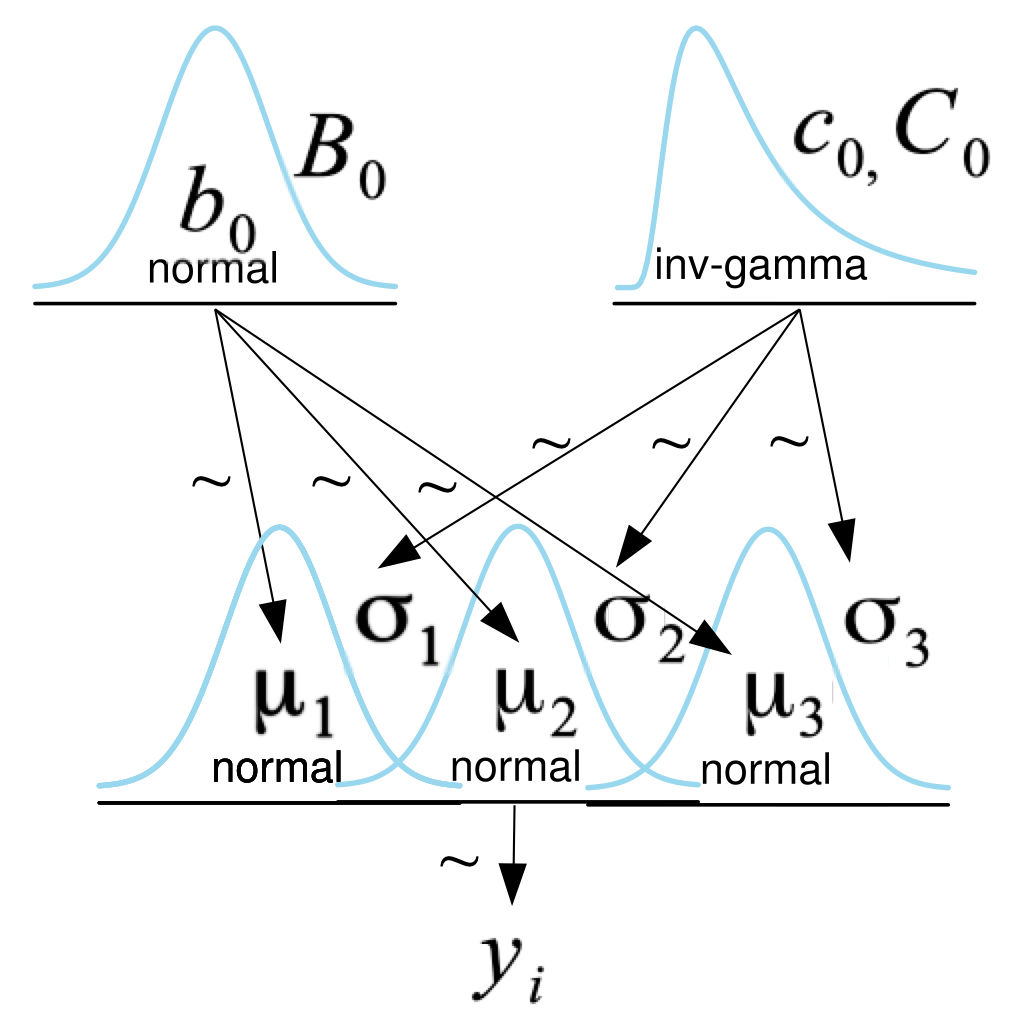
\includegraphics[width=0.5\textwidth]{anovaModel}
        \caption{Three-component Gaussian mixture with known allocations for the Bayesian analysis of variance}
    \label{fig:anovaModel}
\end{figure}
The measured variables $y_i$ follow a three-component Gaussian mixture with known allocations. The first group is normally distributed as $\mathcal{N}(\mu_1,\sigma_1)$, the second group as $\mathcal{N}(\mu_2,\sigma_2)$ and the third group as $\mathcal{N}(\mu_3,\sigma_3)$. The means $\mu_1, \mu_2$ and $\mu_3$ are each distributed as $\mu_j \sim \mathcal{N}(b_0,B_0), j=1,2,3$ with noninformative hyperparameters $b_0$ and $B_0$ and the standard deviations $\sigma_1,\sigma_2$ and $\sigma_3$ are distributed as $\sigma_j \sim \mathcal{G}^{-1}(c_0,C_0), j=1,2,3$ with noninformative hyperparameters $c_0$ and $C_0$. For details, see \cite{Kelter2021StatisticsInBiosciences,Kelter2020JORSBayest}. As the allocations are known, the weights $\eta_1,\eta_2$ and $\eta_3$ are known too, and need not to be estimated, which is why the parameters $\eta_1,\eta_2,\eta_3$ are not included in the diagram. The model visualized in Figure \ref{fig:anovaModel} can be generalized for an arbitrary number of mixture components, which then includes nearly arbitrary ANOVA settings for comparison of multiple groups. A definitive advantage of this model is that inference is obtained for both means and standard deviations, yielding richer information compared to the testing perspectives which are stressed in traditional or Bayesian ANOVA models focussing on the Bayes factor. Also, posterior distributions of effect sizes can be obtained via MCMC, providing an additional layer of information to draw inferences.
	
Instead of relying on the Bayes factor, the \pkg{bayesanova} package follows the approach of \cite{Kruschke2018a} to use a region of practical equivalence (ROPE). The effect size $\delta$ is routinely categorized as small, medium or large in medical research when $\delta \in [0.2,0.5),\delta \in [0.5,0.8)$ or $\delta \in [0.8,\infty)$, see \cite{cohen_statistical_1988}. The approach using the ROPE proceeds by taking these categories as regions of practical equivalence, that is both $\delta=0.25$ and $\delta=0.26$ are identified as a small effect because both are inside the region of practical equivalence $[0.2,0.5)$ of a small effect $\delta$. The underlying idea is that measuring effect sizes only makes sense up to a specific precision, which is given by the above categorization of effect sizes. By studying how much probability mass of the posterior distribution of $\delta$ lies inside some of the above ROPEs $[0.2,0.5)$, $[0.5,0.8)$ and $[0.8,\infty)$ of a small, medium and large positive effect for $\delta$ (negative effects analogue), a continuous statement about the most probable effect size $\delta$ given the data can be made. Kruschke originally advocated to use the location of the 95\% highest-posterior-density (HPD) interval in relation to the ROPE to test whether the null value in the middle of the ROPE should be accepted or rejected for practical purposes. Here, this approach is generalized by switching to the amount of posterior probability mass inside the ROPE. Detailed examples are provided later in this paper.

Table \ref{tab:overview} provides an overview about the four ANOVA models and their purpose.
\begin{widetable}[t!]
\centering
\begin{tabular}{p{3.00cm}p{5.25cm}p{1.50cm}p{2.750cm}}
\toprule
Model           & Purpose & Evidence measure & Computational aspects\\
\midrule
Frequentist ANOVA & Testing the global hypothesis that all samples are drawn from populations with identical means against the alternative & F-statistic and p-value & Analytic solution\\
Bayesian ANOVA of \cite{Rouder2012} & Test the global hypothesis that the effect size vector is zero versus the alternative & Bayes factor & Numerical integration required\\
Bayesian ANOVA of \cite{Kruschke2015} & Estimation of effect sizes between groups via ROPE and 95\% HPD & ROPE & Gibbs sampling in MCMC sampler JAGS (or Stan) required \\
Bayesian ANOVA based on Gaussian mixtures & Estimation of effect sizes between groups via the ROPE and posterior probability mass & ROPE & Gibbs sampling without MCMC sampler JAGS (or Stan) required\\
\bottomrule
\end{tabular}
\caption{\label{tab:overview} Overview about the four ANOVA models}
\end{widetable}
Although it appears that the model of \cite{Kruschke2015} and the Gaussian mixture modeling approach proposed in this paper have the same purpose, they differ in how data $y_i$ are assumed to be generated. In the mixture approach we assume that the sample of $n_j$ participants in group $j$ results from a mixture process, e.g. by flipping a coin, rolling a dice or using any other randomization device (as is the case in clinical trials when assigning patients to groups according to a double-blinded protocol). Thus, the process of data generation is not ``one has collected $n_j$ participants for group j'' but ``the given sample of $n_j$ participants in group j is assumed to be a realization of a mixture process where with probability $\eta_j$ participants are assigned to group $j$''. Importantly, note that the realization of $n_j$ participants in group $j$ for $j=1,...,k$ is expected under the mixture component weight $\eta_j=n_j/n$, but also entirely different group sizes $n_j$ can result under such a mixture. In fact, the weights $\eta_j=n_j/n$ which are assumed to be known are the corresponding maximum-likelihood-estimators of the weight parameters $\eta_j$ given the sample sizes $n_j$ for $j=1,...,k$, but the conceptual focus of the mixture approach is to closely mimic the randomization process researchers follow when conducting a randomized controlled trial. Note further that the model of Kruschke assumes homogeneity of variances in contrast to the Gaussian mixture model, but Kruschke's model can easily be extended to account for heterogeneity of variance, rendering this difference less important. Note that both the frequentist ANOVA and the Bayesian version of \cite{Rouder2012} assume homogeneity of variance across groups.

\section{Package structure and implementation}
The \pkg{bayesanova} package has four functions. These provide (1) the MCMC algorithm for conducting the Bayesian ANOVA in the Gaussian mixture model with known allocations, detailed above, (2) checks of the model assumptions and (3) visualizations of the posterior results for easy interpretation and communication of research results. Visualizations of the posterior mixture components in comparison with the original data are provided by the fourth function. An overview is provided in Table \ref{tab:functions}.

\begin{widetable}[t!]
\centering
\begin{tabular}{lp{11.00cm}}
\toprule
Function           & Description \\
\midrule
\code{bayes.anova} & Main function of the package, conducts the MCMC algorithm to provide full posterior inference in the three-component Gaussian mixture model\\
\code{assumption.check} & Helper function for checking the assumption of normality in each group previous to running a Bayesian ANOVA \\
\code{anovaplot} & Provides multiple visualizations of the results, including posterior distributions, difference in means and standard deviations and effect sizes as well as a full ROPE-analysis \\
\code{post.pred.check} & Provides a posterior predictive check for a fitted Bayesian ANOVA model\\
\bottomrule
\end{tabular}
\caption{\label{tab:functions} Outline of the four main functions implemented in \pkg{bayesanova}}
\end{widetable}

The core function is \code{bayes.anova}, which provides the MCMC algorithm to obtain full posterior inference in a $k$-component Gaussian mixture model shown in Figure \ref{fig:anovaModel} for the special case of $k=3$ components. The function implements a Gibbs sampling algorithm, which iteratively updates 
\begin{enumerate}
	\item{the means $\mu_j|\mu_{-j}, \sigma_1, ..., \sigma_k, S, y$ given the other means $\mu_{-j}$ and standard deviations $\sigma_1, ..., \sigma_k$ as well as the full data $S,y$, where $S$ is the indicator vector for the groups the observations $y$ belong to}
	\item{the standard deviations $\sigma_j|\sigma_{-j}, \mu_1, ..., \mu_k, S, y$ given the other standard deviations $\sigma_{-j}$ and means $\mu_1, ..., \mu_k$ as well as the full data $S,y$, where $S$ is again the indicator vector for the groups the observations $y$ belong to}	
\end{enumerate}
The details of the Gibbs sampler can be found in \cite{Kelter2020JORSBayest,Kelter2021StatisticsInBiosciences}, and the validity of the method follows from standard MCMC theory, see for example \cite{Robert2004}.

The \code{bayes.anova} function takes as input three numerical vectors \code{first}, \code{second} and \code{third}, which correspond to the observed responses in each of the three groups and provides multiple optional parameters:
\begin{example}
bayes.anova(n=10000, first, second, third, 
fourth = NULL, fifth = NULL, sixth = NULL, 
hyperpars="custom", burnin=n/2, sd="sd", q=0.1, ci=0.95)
\end{example}
These are the only mandatory input values, and currently six groups are the limit \pkg{bayesanova} supports. More than three groups can be handed to the function by providing numerical vectors for the parameters \code{fourth}, \code{fifth} and \code{sixth}.

If no other parameters are provided, the function chooses a default of \code{n=10000} Gibbs sampling iterations, where the burn-in of the Markov chains is set to \code{burnin=n/2}, so that the first 5000 iterations are discarded. The default setting uses inference for means $\mu_j$ and standard deviations $\sigma_j$, which is indicated by the parameter \code{sd="sd"}, but inference for variances $\sigma_j^2$ instead of standard deviations $\sigma_j$ can easily be obtained by setting \code{sd="var"}. The credible level for all computed credible intervals defaults to $0.95$, indicated by \code{ci=0.95}. The two remaining parameters \code{hyperpars} and \code{q} define preselected values for the hyperparameters in the prior, to ensure weakly informative priors are used which influence the analysis as little as possible. For details, see \cite{Kelter2020JORSBayest,Kelter2021StatisticsInBiosciences}, but in general these values apply to a broad range of contexts so that changing them is not recommended. Note, that another set of hyperparameters based on \cite{Raftery1996} can be selected via \code{hyperpars="rafterys"}, if desired.

After execution, the function returns a dataframe including four Markov chains for each parameter of the specified size \code{n-burnin}, to make subsequent convergence assessment or post-processing of the MCMC results possible.

The second function is \code{assumption.check}. This function runs a preliminary assumption check on the data, which is recommended before running a Bayesian ANOVA. The model assumptions are normality in each mixture component, so that the \code{assumption.check} function runs Shapiro-Wilk tests to check for normality \citep{shapiro_analysis_1965}. The input parameters are the three numerical vectors \code{x1}, \code{x2} and \code{x3} including the observed responses in the first, second and third group, and the desired confidence level \code{conf.level} for the Shapiro-Wilk tests:
\begin{example}
assumption.check(x1, x2, x3, x4 = NULL, x5 = NULL, x6 = NULL, conf.level=0.95)
\end{example}
The default confidence level is \code{0.95}. More than three groups can easily be added by providing values for \code{x4}, \code{x5} and \code{x6}.

The third function is \code{anovaplot}, which provides a variety of visualizations of results. The function takes as input a dataframe \code{dataframe}, which should be the result of the \code{bayes.anova} function detailed above, a parameter \code{type}, which indicates which visualization is desired, a parameter \code{sd}, which indicates if the provided dataframe includes posterior draws of $\sigma_j$ or $\sigma_j^2$ and last a parameter \code{ci}, which again defined the credible level used in the computations.
\begin{example}
anovaplot(dataframe, type="rope", sd="sd", ci=0.95)
\end{example}
The default values for \code{sd} is \code{"sd"}, and the default credible level is \code{0.95}. The \code{type} parameter takes one of four possible values: (1) \code{type="pars"}, (2) \code{type="diff"}, (3) \code{type="effect"} and (4) \code{type="rope"}. In the first case, posterior distributions of all model parameters are produced, complemented by convergence diagnostics in form of trace plots, autocorrelation plots and the Gelman-Brooks-Rubin shrink factor \citep{Gelman1998}, which should be close to one to indicate convergence to the posterior. In the second case, the posterior distributions of the differences $\mu_i-\mu_j, j\neq i$ of the group means and differences $\sigma_l-\sigma_r, l\neq r$ of the group standard deviations (or variances, if \code{sd="var"} and the dataframe includes posterior draws of the $\sigma_j^2$'s instead of $\sigma_j$'s) are produced, complemented by the same convergence diagnostics. In the third case, the posterior distributions of the effect sizes $\delta_{lr}, l\neq r$ are produced, which are most often of interest in applied research. In this case, posteriors are complemented by the same convergence diagnostics, too. The last and fourth case produces a full ROPE-analysis, which does provide the posteriors of the effect sizes $\delta_{lr}, l\neq r$, but additionally computes a partitioning of the posterior probability mass into the standardized ROPEs of small, medium and large (and no) effect sizes according to \cite{cohen_statistical_1988}, which are the reference standard in medical and psychological research.

The last function \code{post.pred.check} provides a posterior predictive check for a fitted Bayesian ANOVA model against the original data, which is routine in a Bayesian workflow \cite{Gabry2019}.


\section{Illustrations and examples}
This section provides illustrations and a variety of examples, in which the \pkg{bayesanova} package can be used and provides richer information than existing solutions.

\subsection{Tooth growth of guinea pigs treated with vitamin C}
The guinea pig dataset from above is used as a first example. The data are included in the dataset \code{ToothGrowth} in the \pkg{datasets} package which is part of R. First, data is loaded and split into three groups, corresponding to a low, medium and high administered vitamin C dose:
\begin{example}
R> library(datasets)
R> data(ToothGrowth)
R> head(ToothGrowth,n=3)

   len supp dose
1  4.2   VC  0.5
2 11.5   VC  0.5
3  7.3   VC  0.5

R> library(dplyr)
R> library(tidyr)
R> library(bayesanova)
R> grp1 = (ToothGrowth %>% filter(dose==0.5) %>% select(len))$len 
R> grp2 = (ToothGrowth %>% filter(dose==1.0) %>% select(len))$len 
R> grp3 = (ToothGrowth %>% filter(dose==2.0) %>% select(len))$len
\end{example}
Next, we run the assumption checks on the data
\begin{example}
R> assumption.check(grp1, grp2, grp3, conf.level=0.95)

Model assumptions checked. No significant deviations from normality detected. 
Bayesian ANOVA can be run safely.	
\end{example}
\begin{figure}[h!]
\centering
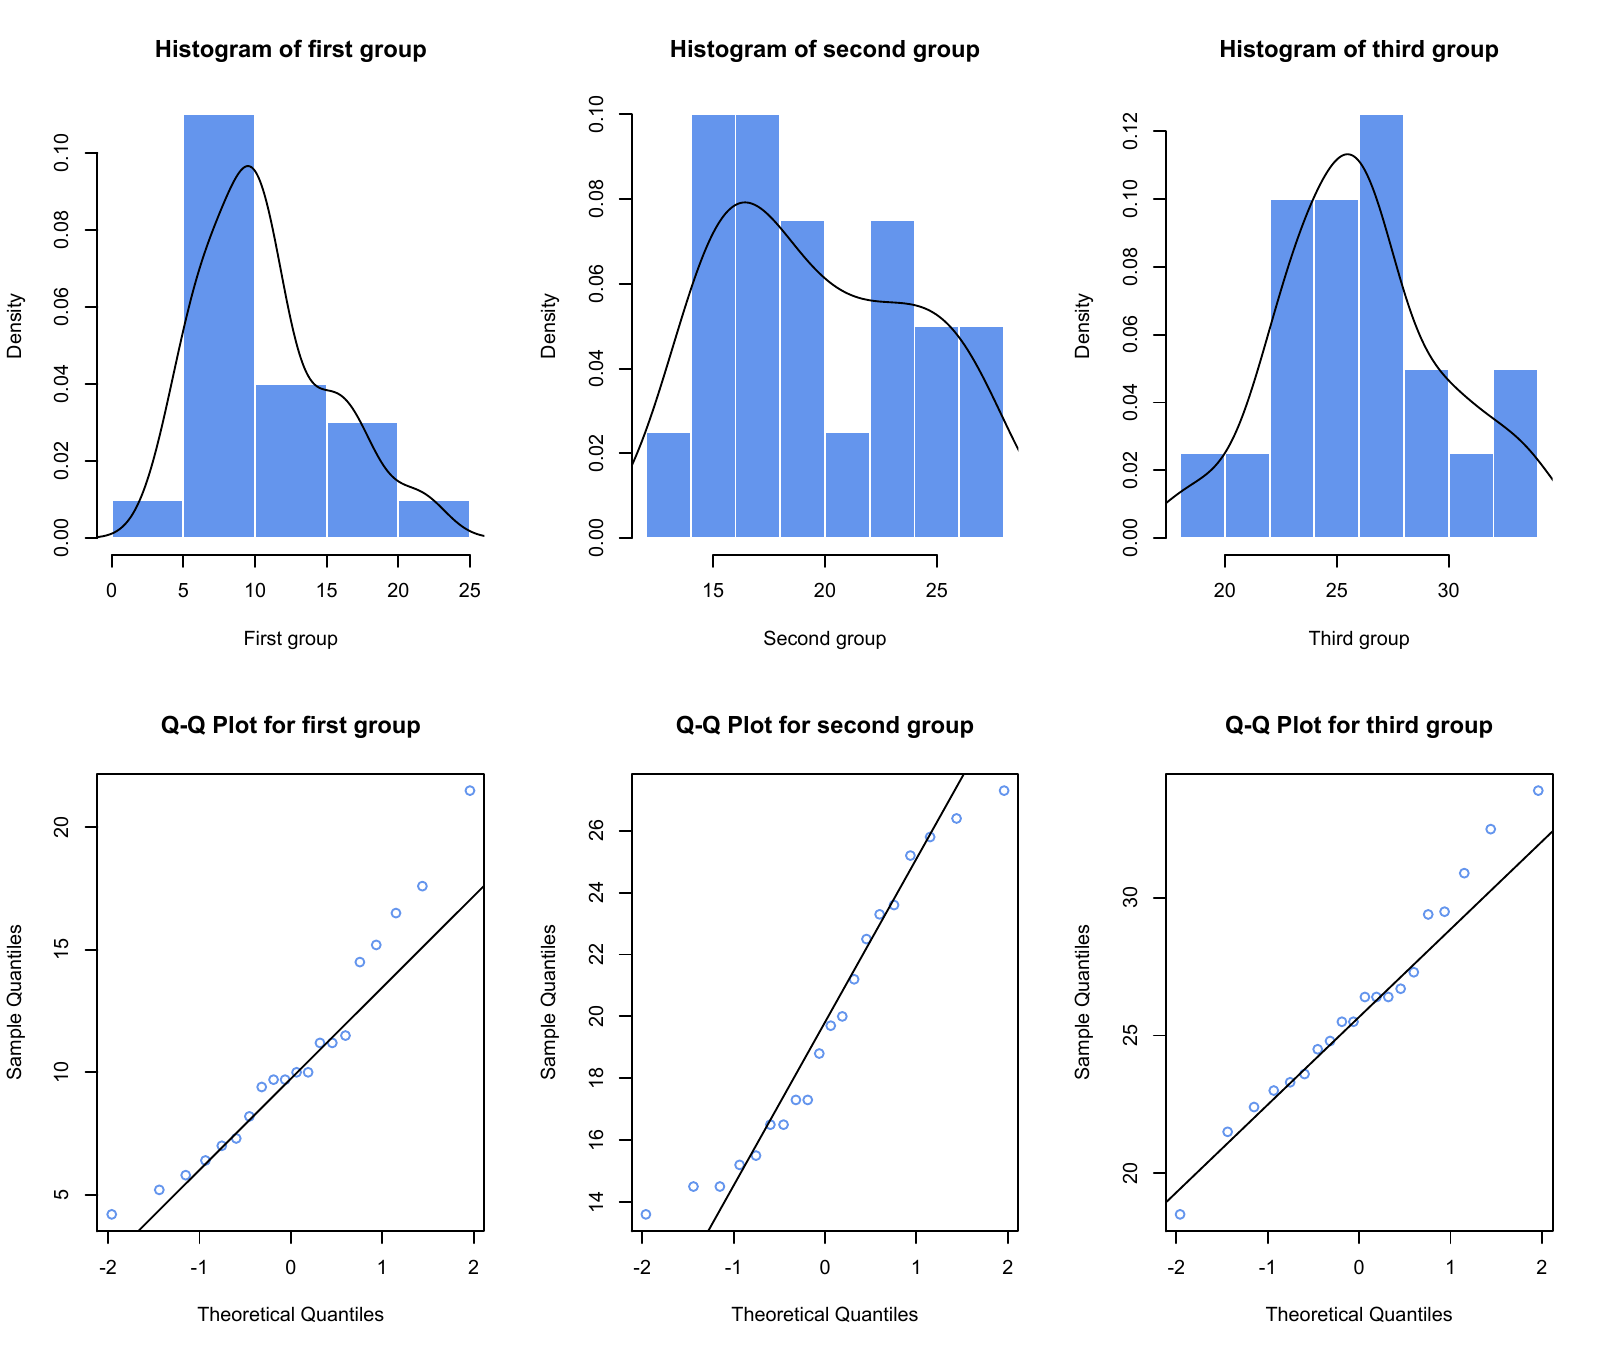
\includegraphics[width=\textwidth]{assumptionsTG}
\caption{Assumption checks for the \code{ToothGrowth} dataset using the \code{assumption.check()} function in \pkg{bayesanova}, showing that data in the three groups can be assumed as normally distributed so that running the Bayesian ANOVA based on the Gaussian mixture model is justified}
\label{fig:assumptionsTG}
\end{figure}
Figure \ref{fig:assumptionsTG} shows the histograms and quantile-quantile plots for all three groups produced by \code{assumption.check()}. Clearly, there are no large deviations, and no Shapiro-Wilk test was significant at the $0.05$ level.

Next, the Bayesian ANOVA can be run via the \code{bayes.anova} function. Therefore, the default parameter values are used, yielding \code{n=5000} posterior draws:
\begin{example}
R> set.seed(42)
R> res = bayes.anova(first = grp1, second = grp2, third = grp3)

|Parameter     |LQ    |Mean  |UQ    |Std.Err |
|:-------------|:-----|:-----|:-----|:-------|
|mu1           |8.69  |10.61 |12.5  |0.91    |
|mu2           |18.05 |19.75 |21.46 |0.84    |
|mu3           |24.94 |26.1  |27.25 |0.57    |
|sigma1        |3.02  |4.07  |5.67  |0.67    |
|sigma2        |2.95  |3.96  |5.43  |0.64    |
|sigma3        |2.43  |3.25  |4.42  |0.52    |
|mu2-mu1       |6.7   |9.15  |11.7  |1.25    |
|mu3-mu1       |13.42 |15.49 |17.67 |1.06    |
|mu3-mu2       |4.36  |6.34  |8.38  |1.01    |
|sigma2-sigma1 |-2.02 |-0.11 |1.68  |0.93    |
|sigma3-sigma1 |-2.62 |-0.81 |0.74  |0.85    |
|sigma3-sigma2 |-2.46 |-0.71 |0.85  |0.82    |
|delta12       |-5.77 |-4.59 |-3.21 |0.65    |
|delta13       |-9.37 |-8.14 |-6.63 |0.71    |
|delta23       |-4.36 |-3.36 |-2.19 |0.56    |
\end{example}
The results table shows the lower and upper quantile, corresponding to the $100\cdot $\code{ci}$+(100-$\code{ci}$)/2$ and $(100-$\code{ci}$)/2$ quantiles where \code{ci} is the credible level chosen above. Also, the posterior mean and standard error are given for each parameter, difference of parameters and effect size.
The results clearly show that there are huge differences between the groups: For example, one can immediately spot that the more vitamin c given, the more tooth growth can be observed via tooth lengths. While the first group (low dose) has a posterior mean of $10.61$ with credible interval $[8.69,10.61]$, the second group achieves a mean of $19.75$ with credible interval $[18.05,21.46]$. The third group has a posterior mean of even $26.1$ with credible level $[24.94.27.25]$. The posterior estimates for the differences $\mu_2-\mu_1$, $\mu_3-\mu_1$ and $\mu_3-\mu_2$ show that all groups differ from each other with a very high probability, given the data.

Note that the information provided is much more fine-grained than in the solutions via the traditional ANOVA and the Jeffreys-Zellner-Siow based Bayes-factor ANOVA above. While in these two solutions, one could only infer that the model using both predictors and the interaction term is the best, now we are given precise estimates of the effect sizes between each group defined by the dose of vitamin c administered. Note also, that including the second predictor \code{supp} is no problem, leading to a setting which incorporates six groups in the mixture then.

\subsection{Heart rate data for runners}
The second example is from the biomedical sciences and uses the heart rate data from \cite{Moore2012}. In the study, heart rates of female and male runners and generally sedentary participants (not regularly running) following six minutes of exercise were recorded. The participant's \code{Gender} and \code{Heart.rate} are given and which group he or she belongs to (\code{Group=="Runners"} or \code{Group=="Control"}). In the study, 800 participants were recruited, so that in each of the four groups given by the combinations of \code{Gender} and \code{Group} 200 subjects participated.

Therefore, the situation requires a $2\times 2$ between subjects ANOVA. Specifically, interest lies in the hypothesis that heart rate differs between gender and groups. The Bayesian ANOVA of \pkg{bayesanova} can easily be applied in such an often encountered setting. We first load the data and split them into the four groups:
\begin{example}
R> library(dplyr)
R> hr=read.csv("heartrate.csv",sep=",")
R> head(hr)

  Gender   Group Heart.Rate
1 Female Runners        119
2 Female Runners         84
3 Female Runners         89
4 Female Runners        119
5 Female Runners        127
6 Female Runners        111

R> femaleRunners = (hr %>% filter(Gender=="Female") 
+  %>% filter(Group=="Runners")  
+  %>% select(Heart.Rate))$Heart.Rate
R> maleRunners = (hr %>% filter(Gender=="Male") %>% filter(Group=="Runners") 
+  %>% select(Heart.Rate))$Heart.Rate
R> femaleControl = (hr %>% filter(Gender=="Female") 
+  %>% filter(Group=="Control")  
+  %>% select(Heart.Rate))$Heart.Rate
R> maleControl = (hr %>% filter(Gender=="Male") %>% filter(Group=="Control")
+  %>% select(Heart.Rate))$Heart.Rate
\end{example}

Then, we check the model assumptions:
\begin{example}
R> assumption.check(femaleRunners, maleRunners, femaleControl, maleControl)
\end{example}
We can thus safely proceed running the Bayesian ANOVA:
\begin{example}
R> set.seed(42)
R> resRunners = bayes.anova(first = femaleRunners, second = maleRunners, 
+  third = femaleControl, fourth = maleControl)

|Parameter     |LQ     |Mean   |UQ     |Std.Err |
|:-------------|:------|:------|:------|:-------|
|mu1           |113.48 |116    |118.5  |1.27    |
|mu2           |102.51 |103.98 |105.55 |0.76    |
|mu3           |145.44 |148.04 |150.52 |1.3     |
|mu4           |127.12 |130.01 |132.82 |1.47    |
|sigma1        |14.38  |15.87  |17.51  |0.8     |
|sigma2        |11.21  |12.35  |13.67  |0.63    |
|sigma3        |14.71  |16.19  |17.85  |0.82    |
|sigma4        |15.46  |17.02  |18.79  |0.85    |
|mu2-mu1       |-14.9  |-12.01 |-9.06  |1.48    |
|mu3-mu1       |28.47  |32.04  |35.6   |1.83    |
|mu4-mu1       |10.19  |14.01  |17.9   |1.96    |
|mu3-mu2       |41.12  |44.05  |46.95  |1.51    |
|mu4-mu2       |22.83  |26.02  |29.21  |1.66    |
|mu4-mu3       |-21.8  |-18.03 |-14.4  |1.92    |
|sigma2-sigma1 |-5.6   |-3.52  |-1.57  |1.02    |
|sigma3-sigma1 |-1.94  |0.32   |2.53   |1.15    |
|sigma4-sigma1 |-1.14  |1.15   |3.51   |1.18    |
|sigma3-sigma2 |1.83   |3.84   |5.85   |1.03    |
|sigma4-sigma2 |2.7    |4.67   |6.8    |1.05    |
|sigma4-sigma3 |-1.48  |0.83   |3.13   |1.17    |
|delta12       |2.4    |3.2    |3.96   |0.4     |
|delta13       |-8.92  |-8.01  |-7.05  |0.48    |
|delta14       |-4.42  |-3.46  |-2.5   |0.49    |
|delta23       |-12.55 |-11.67 |-10.77 |0.45    |
|delta24       |-7.65  |-6.79  |-5.91  |0.45    |
|delta34       |3.52   |4.43   |5.37   |0.48    |
\end{example}

The results reveal multiple insights now. To support the interpretation, we first produce visualisations of the results via the \code{anovaplot()} function:
\begin{example}
R> anovaplot(resRunners)
\end{example}
Figure \ref{fig:plotHR1} shows the plots produces by the above call to \code{anovaplot()}. 
\begin{figure}[h!]
\centering
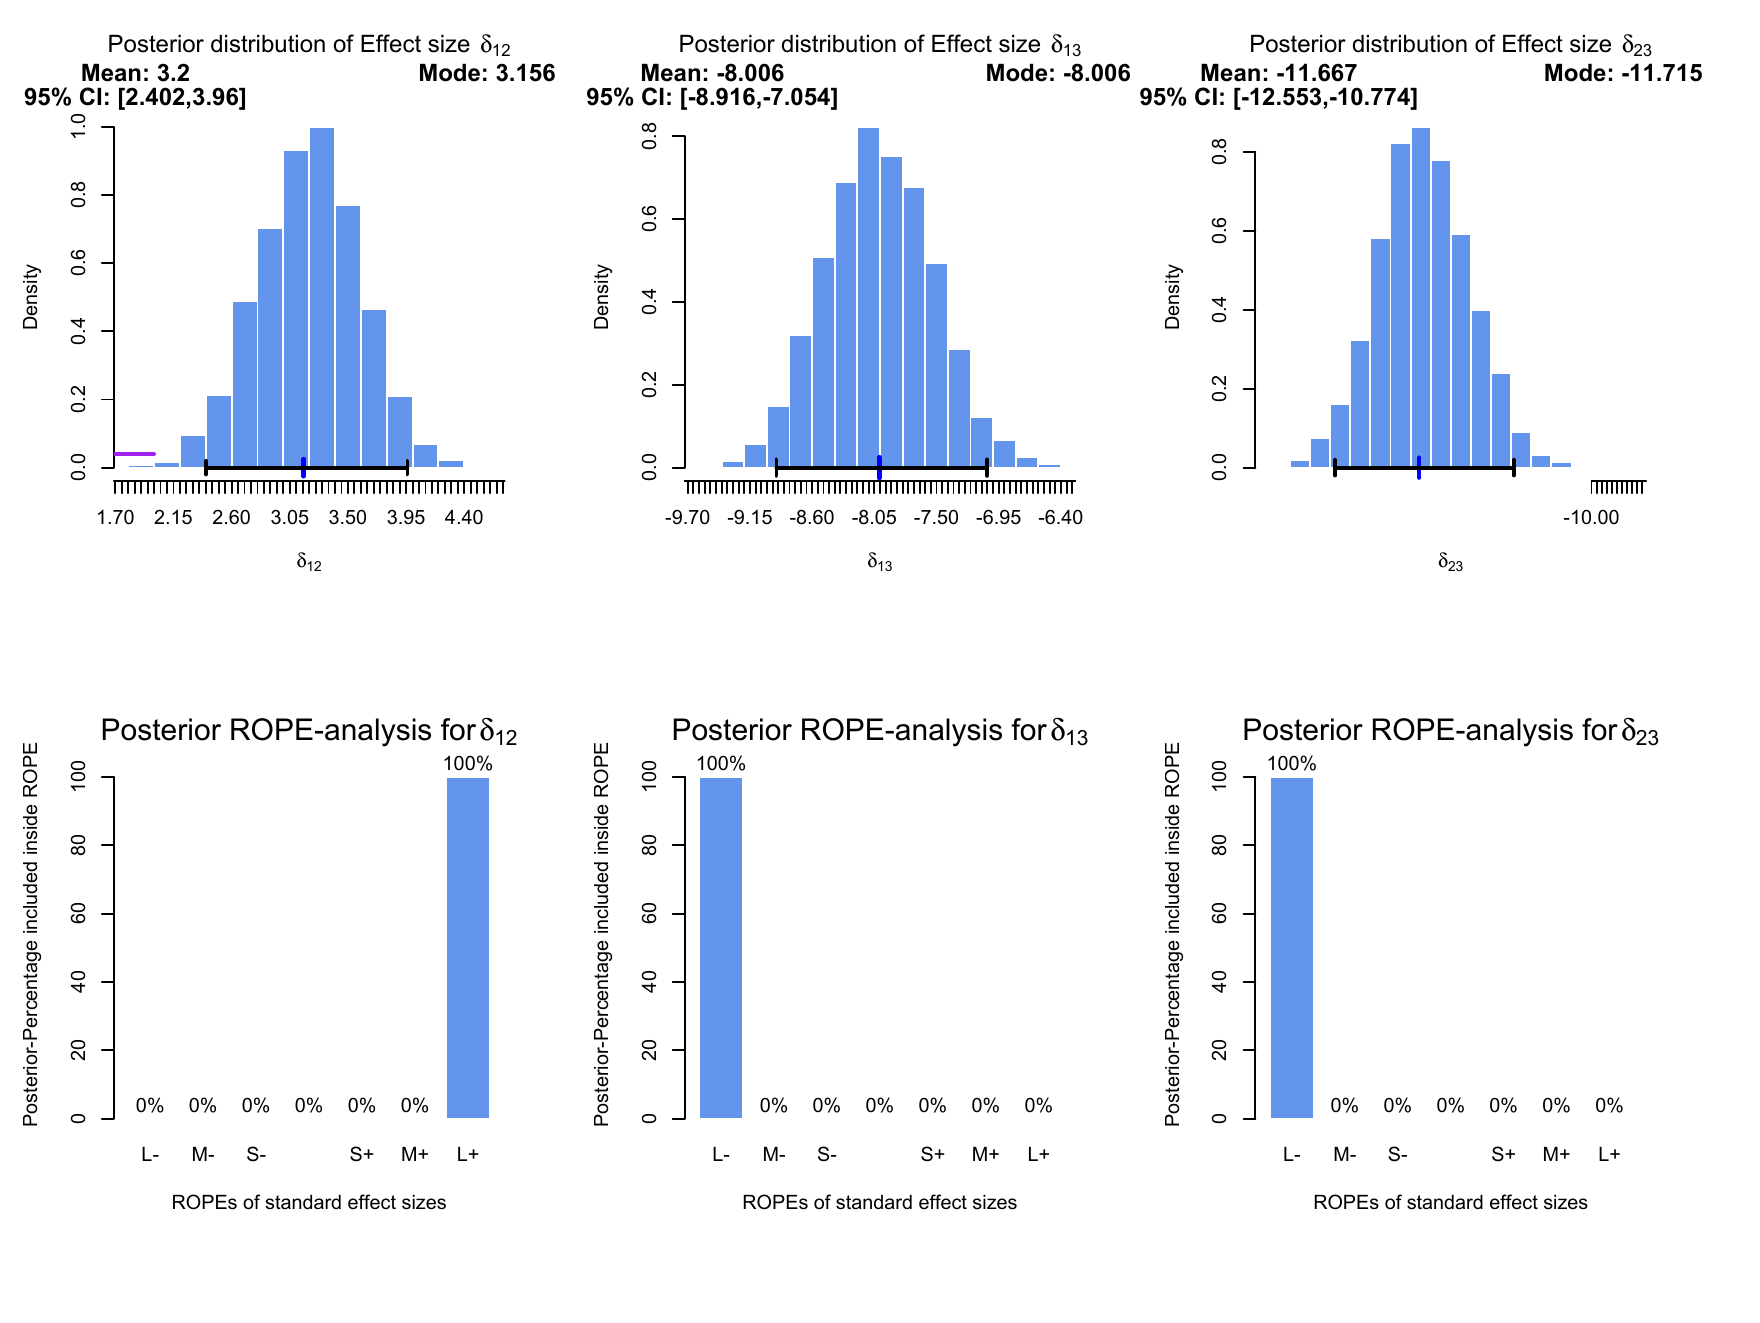
\includegraphics[width=0.85\textwidth]{plotHR1}
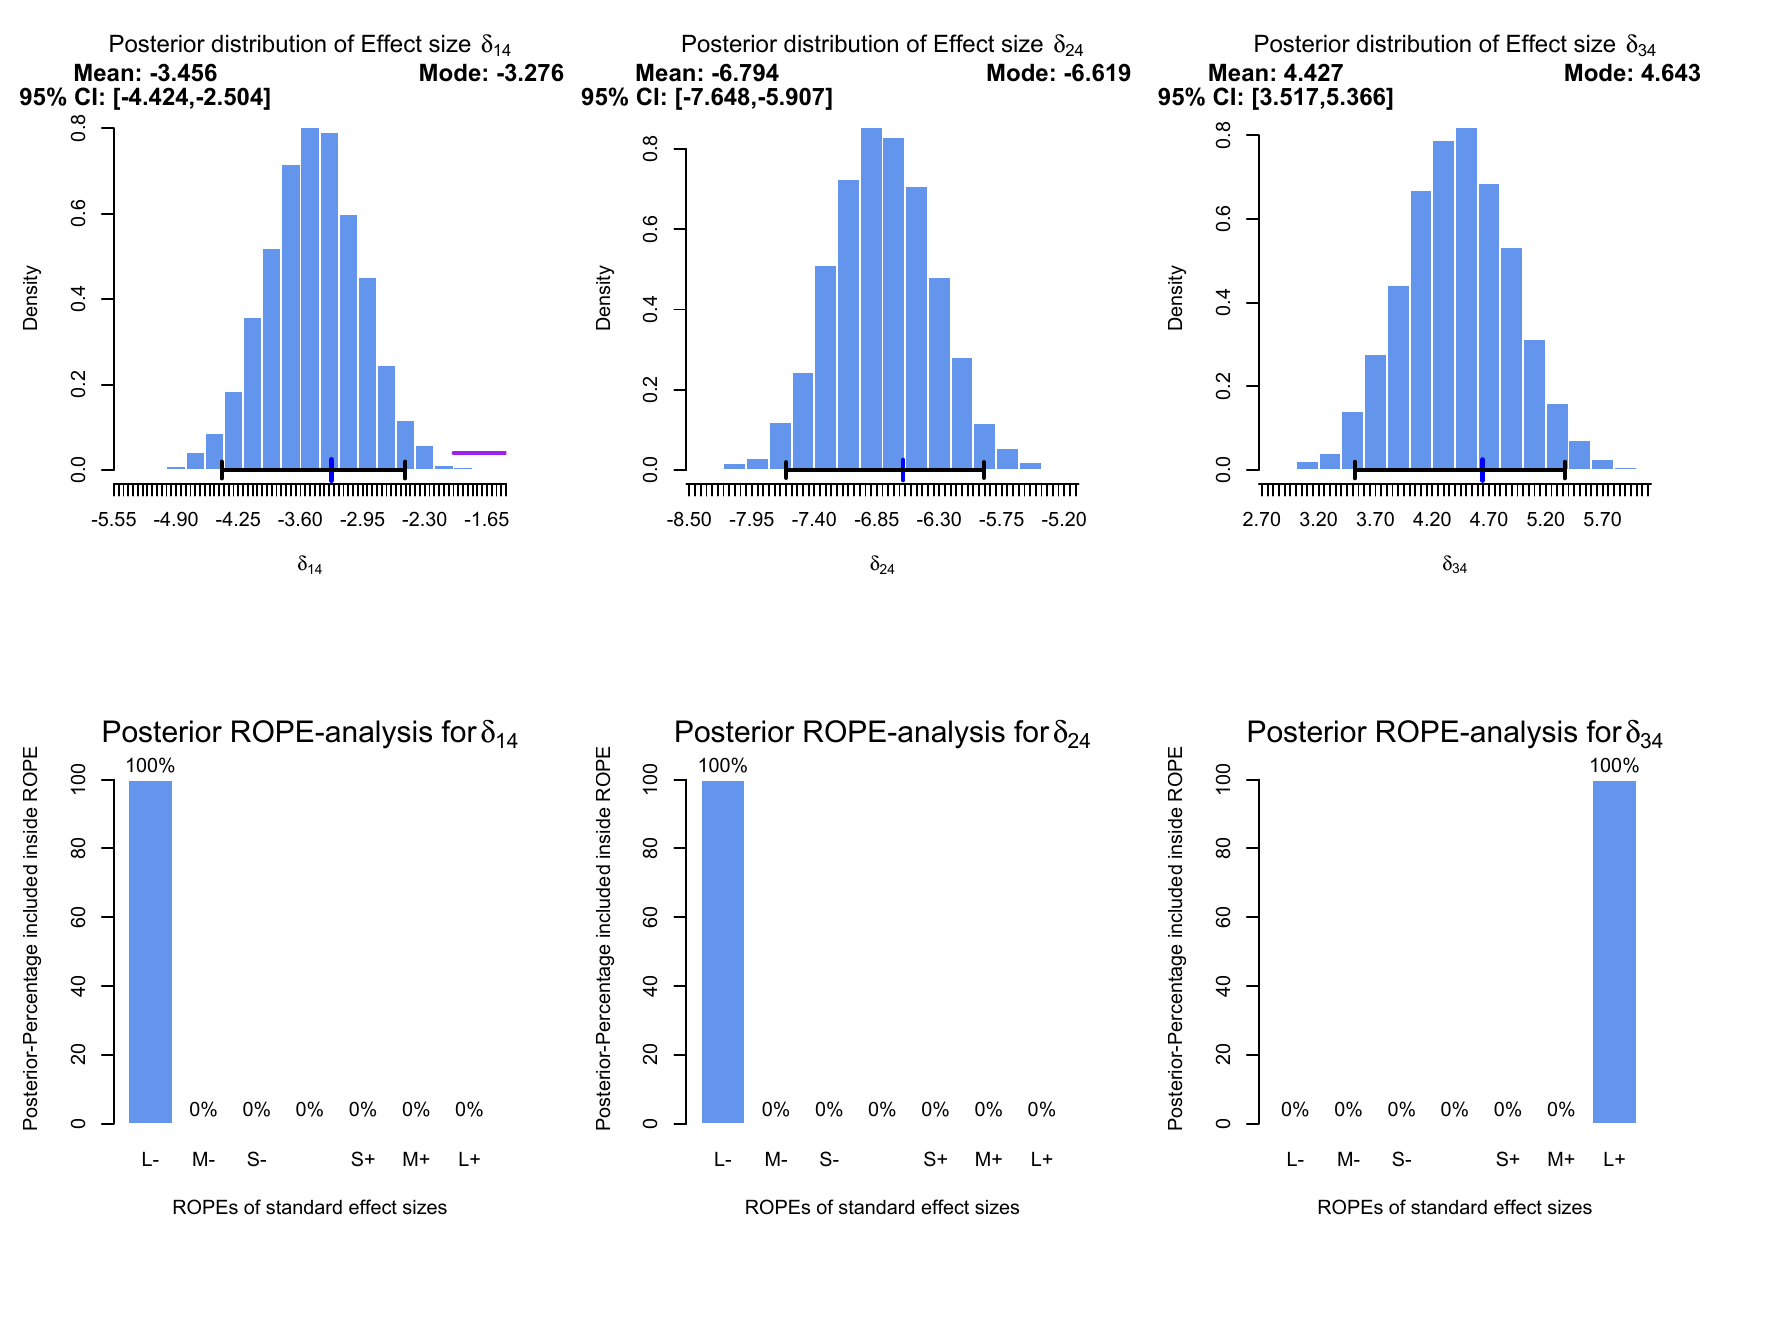
\includegraphics[width=0.85\textwidth]{plotHR2}
\caption{Visualisations of the results for the \code{Heart rate} dataset using the \code{anovaplot()} function in \pkg{bayesanova}, showing (1) the resulting posterior distributions of the effect sizes between each pair of groups (first and third row) and (2) the posterior ROPE-analysis for each group comparison (second and fourth row)}
\label{fig:plotHR1}
\end{figure}
The first row shows the posterior distributions of the effect sizes $\delta_{12}$, $\delta_{13}$ and $\delta_{23}$. The second row below is the analysis based on the ROPE, which partitions the posterior probability mass into the standard ROPES for effect sizes according to \cite{cohen_statistical_1988}. 

Thus, we can see that for $\delta_{12}$ -- which equals the effect size between female runners and male runners -- there is a very large effect with posterior mean $3.2$ and 95\% credible interval $[2.402,3.96]$, confirmed by the fact that $100\%$ of the posterior probability mass are located inside the ROPE of a large effect according to \cite{cohen_statistical_1988} (which includes values $\geq 0.8$). Based on the results, the posterior probability of a large effect between female and male runners given the data is one, which means female runners have a faster heart beat after exercising six minutes than male runners. 

To check if this effect exists also in the control groups, we compare the posterior of $\delta_{34}$, corresponding to the effect size between the female and male controls. The results are given in the right plot of the third and fourth row in  \ref{fig:plotHR1} and show that also in the control groups the effect is present. Here, the effect size is estimated to be even larger than for the runner groups with a posterior mean of $4.427$ and a 95\% credible interval $[3.517,5.366]$. Thus, regular running seems to reduce the observed heartbeat differences between males and females in the form of a large effect. We could proceed this way and compare all other groups, too.

To check the model fit, we use the \code{post.pred.check} function, which performs a posterior predictive check against the observed data by drawing \code{reps} samples from the posterior distribution and visualizing the original data's density with density overlays for the reps sampled posterior predictive densities of the data:
\begin{example}
post.pred.check(anovafit = resRunners, ngroups = 4, out = hr$Heart.Rate , 
reps = 50, eta = c(1/4,1/4,1/4,1/4))	
\end{example}
The argument \code{anovafit} takes the resulting dataframe of the \code{bayes.anova} function as input, the number of groups is specified in \code{ngroups}, \code{out} is the vector of all data originally observed (no matter which group), \code{reps} is the number of posterior predictive density overlays desired, and \code{eta} is the vector of weights used in the Gaussian mixture. Here, as all four groups include 200 participants, each weight is $1/4$. The resulting posterior predictive check is shown in the left plot of  \ref{fig:ppchecks}, and indicates that while there is some overdispersion in the center of the posterior predictive distributions simulated, the overall fit seems reasonable.
\begin{figure}[h!]
\centering
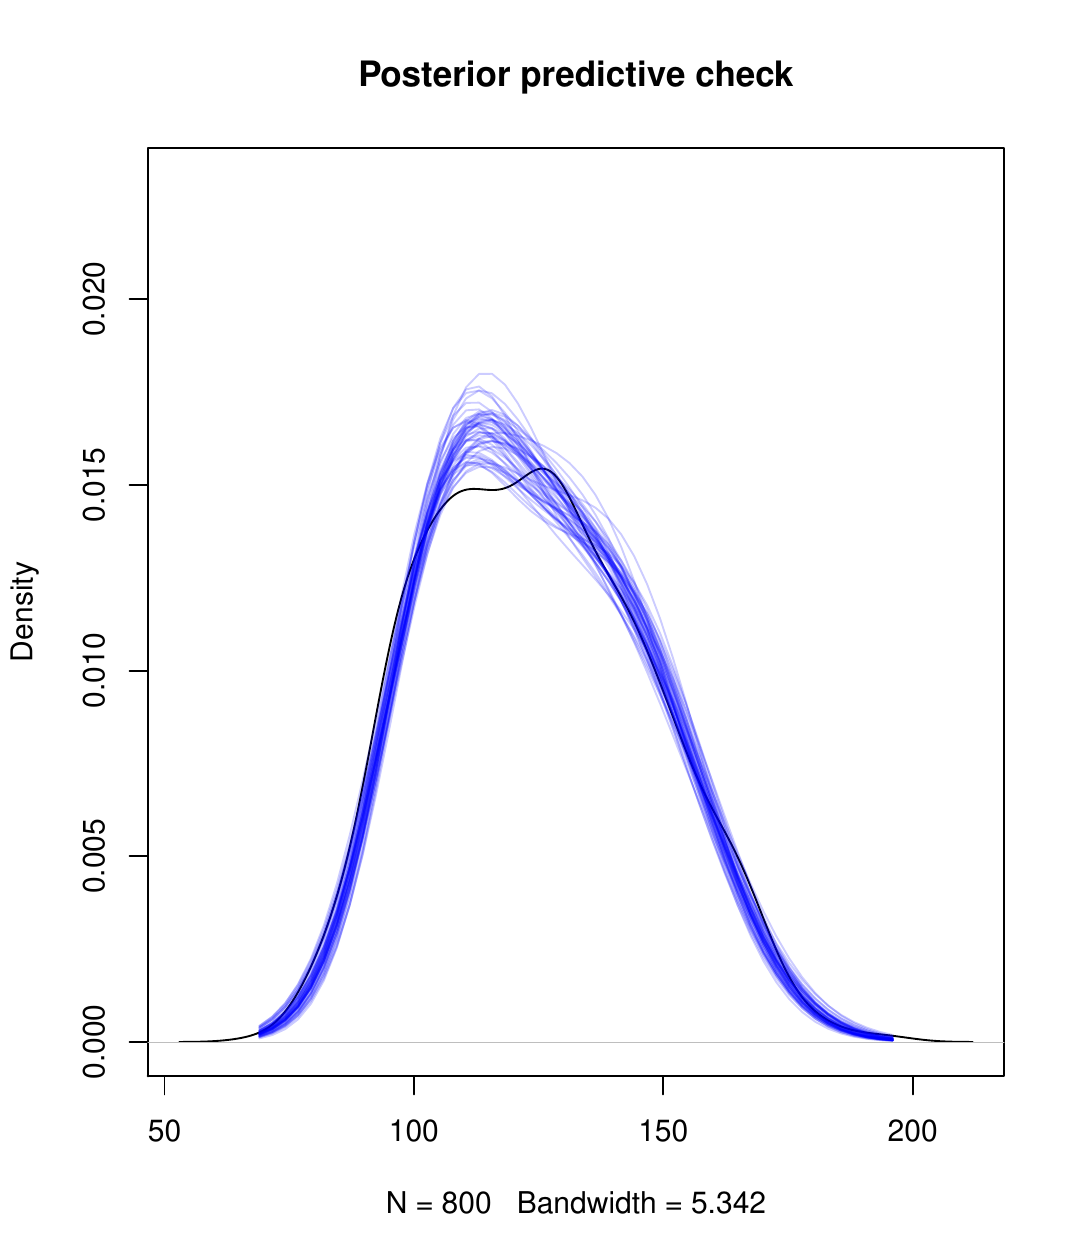
\includegraphics[width=0.45\textwidth]{ppcheckRunners}
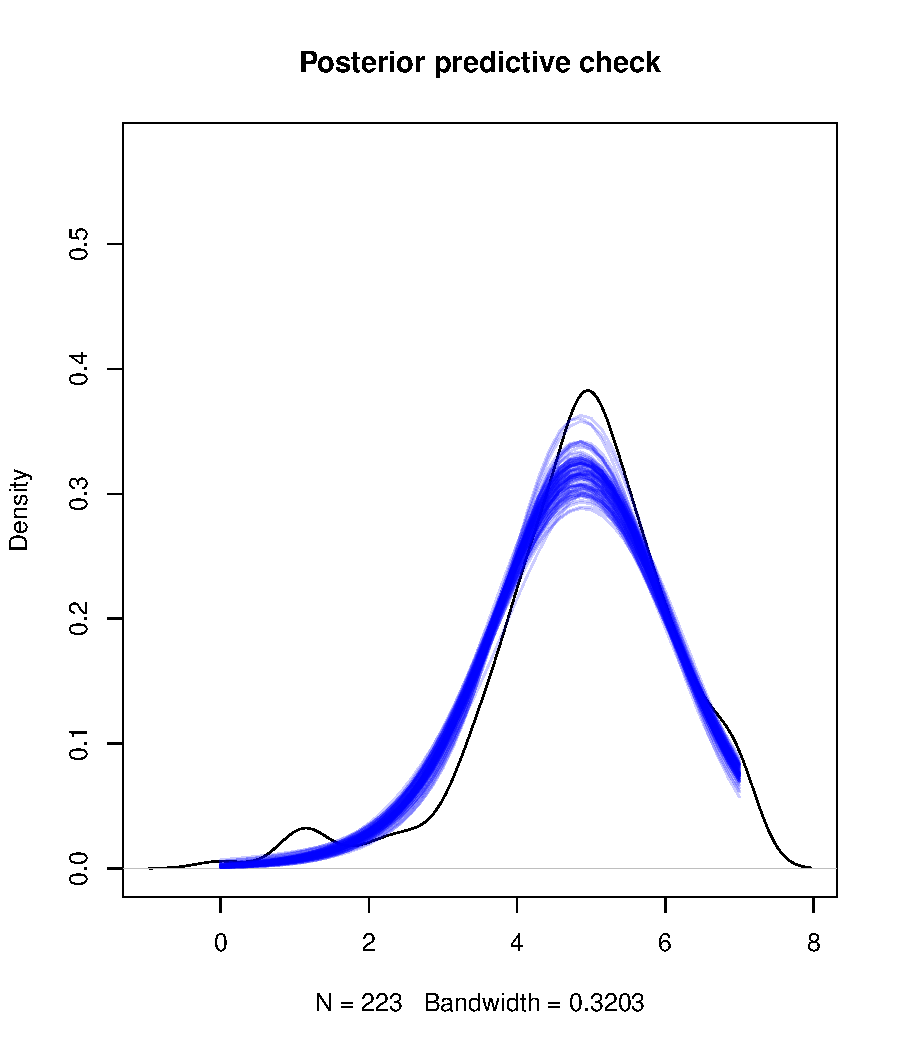
\includegraphics[width=0.45\textwidth]{ppcheckFeelings}
\caption{Posterior predictive checks using the \code{post.pred.check} function; left: For the \code{runners} dataset; right: For the \code{feelings} dataset; in both cases, results show that the overall fit of the Gaussian mixture model is reasonable}
\label{fig:ppchecks}
\end{figure}


\subsection{Pleasantness ratings after watching artistic or nude pictures}
This example uses data from a study conducted by \cite{Balzarini2017}, in which men and women's feelings towards their partners after watching either erotic or abstract art pictures were analysed. The study was published in the \textit{Journal of Experimental Social Psychology}, and also the average pleasantness obtained from viewing the pictures was studied, as one of the research questions was whether men and women rate pleasantness of the pictures differently for nude and abstract art. This leads to a $2\times 2$ factorial ANOVA for the variables gender and picture type, coded as \code{Gender} and \code{Condition} in the dataframe.

First, data is loaded and split into the four groups of interest:
\begin{example}
R> feelings=read.csv("feelings.csv",sep=",")
R> head(feelings)

  Gender Age  RelLen    Condition PartnerAttractiveness
1   Male  43  3.7500        Nudes                    21
2 Female  26  3.0000        Nudes                    19
3 Female  35  5.2500 Abstract Art                    27
4 Female  31  2.0000 Abstract Art                    22
5 Female  23  4.0000 Abstract Art                    27
6   Male  36 19.9167        Nudes                    16
  LoveForPartner AveragePleasantness
1             76              5.9375
2             66              4.7500
3            103              6.2500
4             76              5.5625
5            109              2.3750
6             98              5.1250

R> femaleArtistic = (feelings %>% filter(Gender=="Female") %>% 
+  filter(Condition=="Abstract Art"))$AveragePleasantness
R> maleArtistic = (feelings %>% filter(Gender=="Male") %>% 
+  filter(Condition=="Abstract Art"))$AveragePleasantness
R> femaleNude = (feelings %>% filter(Gender=="Female") %>% 
+  filter(Condition=="Nudes"))$AveragePleasantness
R> maleNude = (feelings %>% filter(Gender=="Male") %>% 
+  filter(Condition=="Nudes"))$AveragePleasantness
\end{example}
Second, the model assumption of normality in each group is checked:
\begin{example}
R> assumption.check(femaleArtistic, maleArtistic, femaleNude, maleNude)

1: In assumption.check(femaleArtistic, maleArtistic, femaleNude, maleNude) :
  Model assumption of normally distributed data in each group is violated.
 All results of the Bayesian ANOVA based on a Gaussian mixture 
 could therefore be unreliable and not trustworthy.
2: In assumption.check(femaleArtistic, maleArtistic, femaleNude, maleNude) :
  Run further diagnostics (like Quantile-Quantile-plots) to check if the 
  Bayesian ANOVA can be expected to be robust to the violations of normality	
\end{example}
This time the function gives a warning, that there are violations of the distributional assumptions. Investigating the results leads to the conclusion that data in the fourth group deviate from normality, shown in  \ref{fig:histPL} in the QQ-plot. Still, as all other groups show no strong deviations from normality, we proceed and are cautious when drawing inferences including any statements involving the fourth group.
\begin{figure}[h!]
\centering
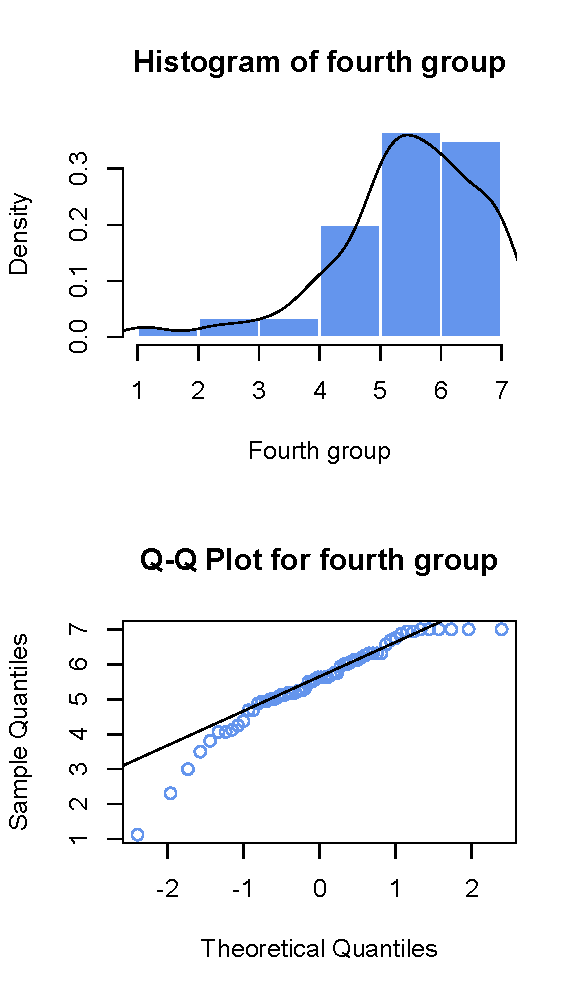
\includegraphics[width=0.4\textwidth]{histPL}
\caption{Histogram and quantile-quantile plot for the fourth group in the \code{feelings} dataset, showing that the assumption of normality is violated}
\label{fig:histPL}
\end{figure}

Keeping this in mind, the Bayesian ANOVA is run now with default hyperparameters:
\begin{example}
R> set.seed(42)
R> resFeelings = bayes.anova(first = femaleArtistic, second = maleArtistic,
+   third = femaleNude, fourth = maleNude)

|Parameter     |LQ    |Mean  |UQ    |Std.Err |
|:-------------|:-----|:-----|:-----|:-------|
|mu1           |4.86  |4.9   |4.95  |0.02    |
|mu2           |4.62  |4.66  |4.69  |0.02    |
|mu3           |4.07  |4.2   |4.34  |0.07    |
|mu4           |5.42  |5.47  |5.53  |0.03    |
|sigma1        |0.98  |1.16  |1.4   |0.11    |
|sigma2        |0.86  |1.02  |1.21  |0.09    |
|sigma3        |1.34  |1.66  |2.06  |0.19    |
|sigma4        |1.06  |1.26  |1.52  |0.12    |
|mu2-mu1       |-0.31 |-0.25 |-0.19 |0.03    |
|mu3-mu1       |-0.85 |-0.7  |-0.56 |0.07    |
|mu4-mu1       |0.5   |0.57  |0.64  |0.04    |
|mu3-mu2       |-0.6  |-0.46 |-0.32 |0.07    |
|mu4-mu2       |0.75  |0.81  |0.87  |0.03    |
|mu4-mu3       |1.12  |1.27  |1.41  |0.07    |
|sigma2-sigma1 |-0.43 |-0.14 |0.12  |0.14    |
|sigma3-sigma1 |0.1   |0.49  |0.95  |0.21    |
|sigma4-sigma1 |-0.21 |0.1   |0.42  |0.16    |
|sigma3-sigma2 |0.27  |0.64  |1.07  |0.21    |
|sigma4-sigma2 |-0.04 |0.24  |0.55  |0.15    |
|sigma4-sigma3 |-0.84 |-0.39 |0.01  |0.22    |
|delta12       |0.18  |0.24  |0.29  |0.03    |
|delta13       |0.47  |0.6   |0.73  |0.07    |
|delta14       |-0.58 |-0.52 |-0.44 |0.04    |
|delta23       |0.27  |0.41  |0.53  |0.06    |
|delta24       |-0.84 |-0.76 |-0.69 |0.04    |
|delta34       |-1.2  |-1.07 |-0.91 |0.07    |
\end{example}
The results show that differences are now much more subtle than in the previous examples. From the results one can spot that the means in the first three groups are located nearer to each other than in the previous examples, and the fourth group differs more strongly from the first three. The standard deviations do not differ a lot between groups, and the magnitude of the posterior effect sizes is now smaller, too. To investigate the effect sizes, visualisations are produced first:
\begin{example}
R> anovaplot(resFeelings)
\end{example}
 
\begin{figure}[h!]
\centering
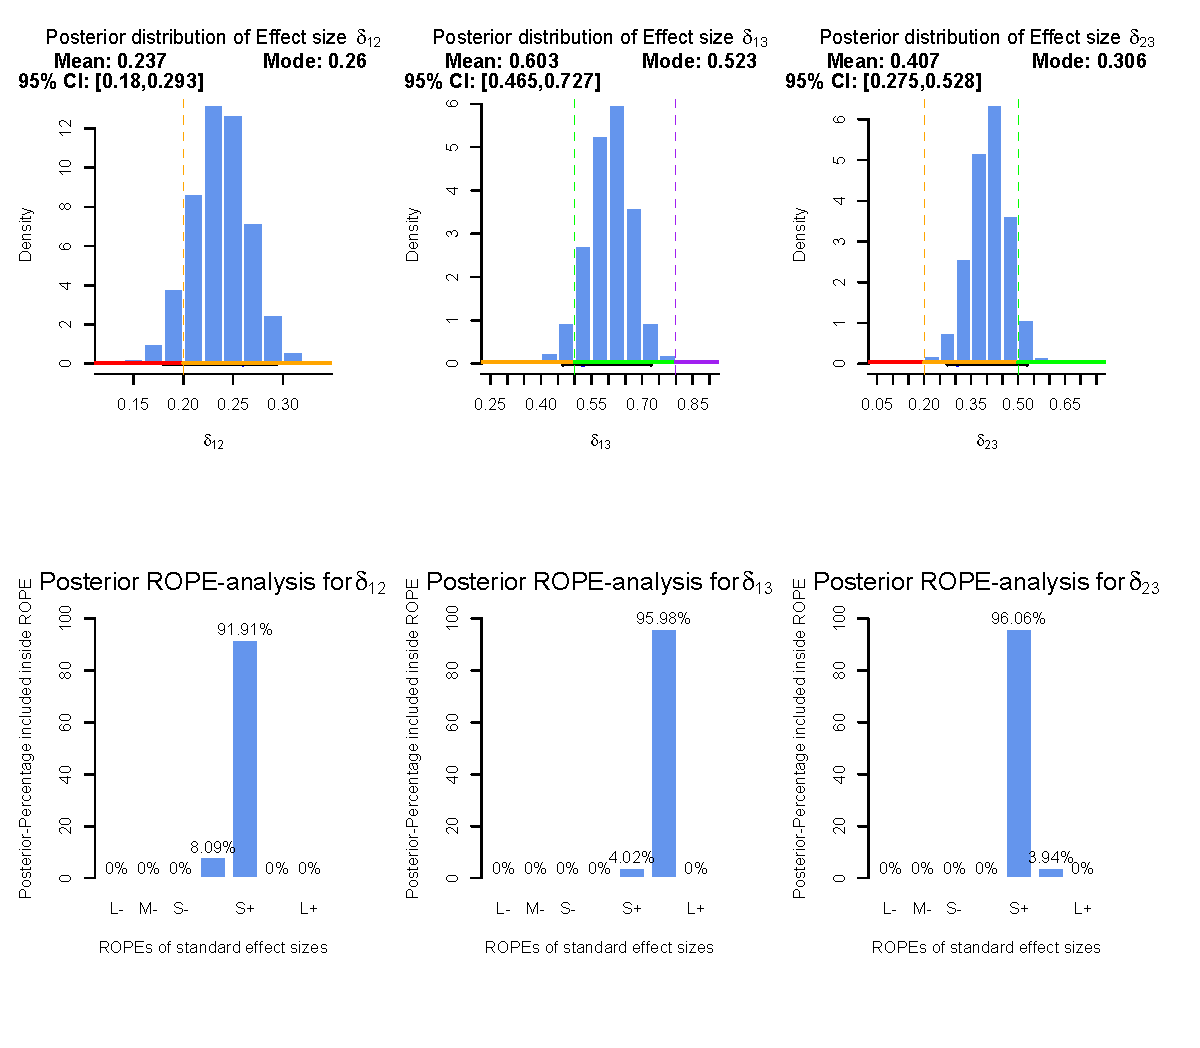
\includegraphics[width=1\textwidth]{histFL2}
\caption{Visualisations of the posterior effect sizes for the \code{feelings} dataset using the \code{anovaplot()} function in \pkg{bayesanova}, showing which effects are most probable a posteriori based on a ROPE-analysis for each pair of groups}
\label{fig:plotFL1}
\end{figure}
Figure \ref{fig:plotFL1} shows the plots produces by the above call to \code{anovaplot()}. The two left plots show that with $91.91$\% probability there is a small effect between the first and second group given the data, which are the female and male artistic pictures groups. Therefore, with large probability females rate artistic pictures more pleasant than males, where the effect size itself is small. Still, we could argue that there is nonnegligible probability of $8.09$\% that there is no effect at all and therefore not draw any conclusion depending on the posterior probability we require. 

The middle two plots in  \ref{fig:plotFL1} show the effect between the female artistic and female nude picture groups. We can see that based on the posterior distribution of $\delta_{13}$, with $95.98$\% there is a medium effect between the two groups given the data. Females rate artistic pictures therefore with a probability near certainty as more pleasant than nude pictures, where the effect size in terms of standardized differences between ratings is medium.

The right two plots in  \ref{fig:plotFL1} show the effect between the male artistic and female nude groups. The posterior reveals that $96.06$\% indicate a small effect, which could be interpreted as the fact that males rate artistic pictures even more pleasant than females rate nude pictures, but the effect size is only small and the remaining 3.94\% posterior probability indicate that there is even a medium effect.

Figure \ref{fig:plotFL2} shows the effects which include the fourth group. Due to the violations of distributional assumptions one need to be cautious now, as the results could be deterred. Still, the two right plots show the effect size between the female and male nude groups, and indicate that the full posterior (100\%) signals a large negative effect. This means, males rate the pleasantness of nude pictures much higher than females. Still, the result (as well as the results for $\delta_{14}$ and $\delta_{24}$) are questionable due to the violation of model assumptions, so we do not proceed here.

The posterior predictive check in the right plot of  \ref{fig:ppchecks} obtained via
\begin{example}
post.pred.check(anovafit = resFeelings, ngroups = 4, out = feelings$AveragePleasantness, 
reps = 100, eta = c(58/223,64/223,41/223,60/223))
\end{example}
shows that the overall fit seems reasonable, although there is some room for improvement in the range of average pleasantness ratings between zero and two, and in the peak between average pleasantness ratings of four and six. Subdividing the data even further and refitting the ANOVA model with a higher number of components would be an option to improve the fit. Alternatively, one could discuss the prior hyperparameters chosen here.

\begin{figure}[h!]
\centering
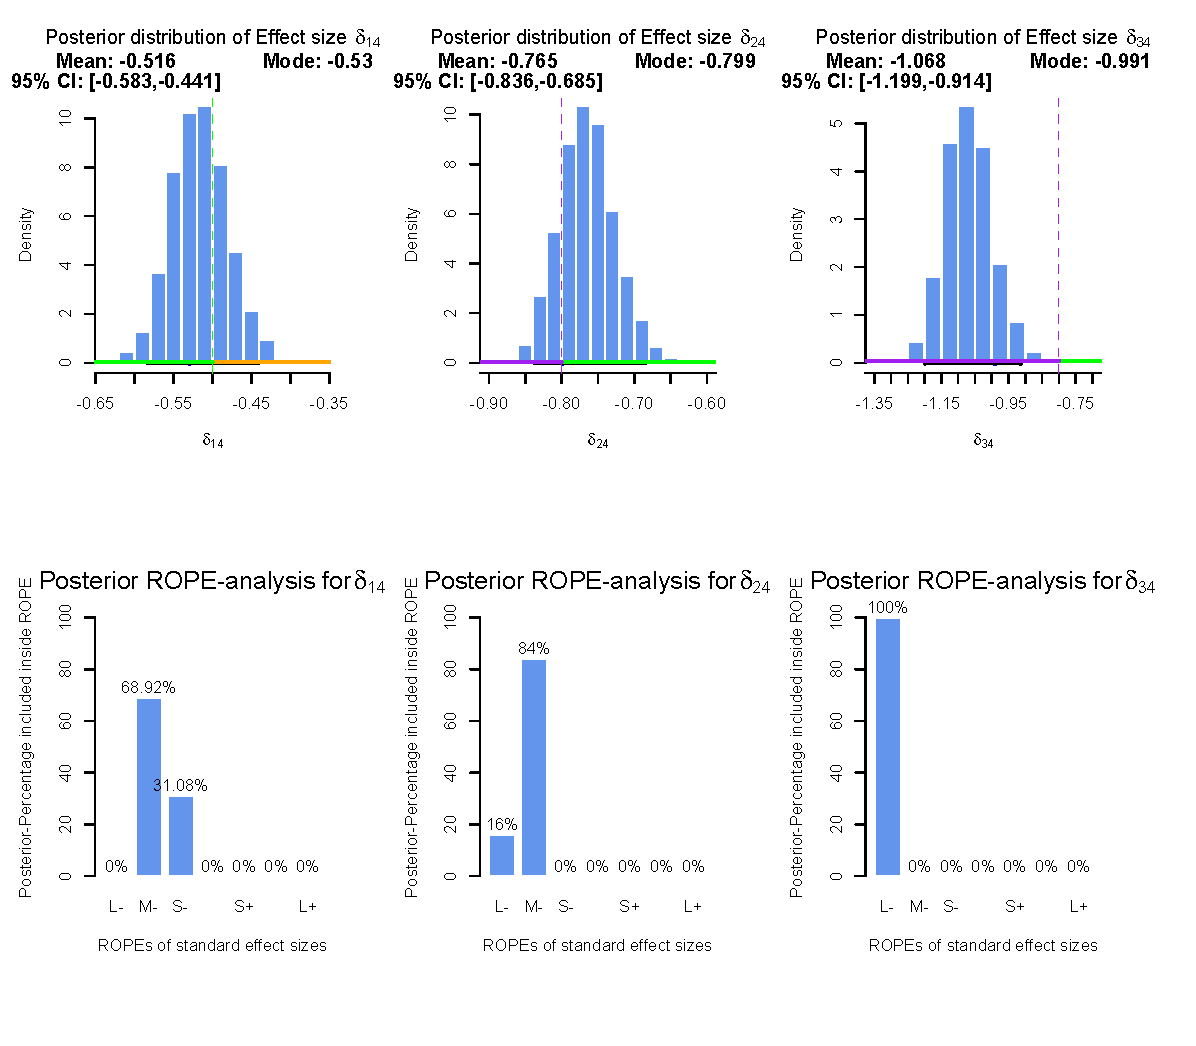
\includegraphics[width=1\textwidth]{histFL1}
\caption{Visualisations of the posterior effect sizes for the \code{feelings} dataset using the \code{anovaplot()} function in \pkg{bayesanova}, showing which effects are most probable a posteriori based on a ROPE-analysis for each pair of groups}
\label{fig:plotFL2}
\end{figure}

A solution via a traditional ANOVA in this case would yield:
\begin{example}
R> summary(aov(AveragePleasantness ~ Gender * Condition, data = feelings))

                  Df Sum Sq Mean Sq F value   Pr(>F)    
Gender             1  10.63  10.629   7.605  0.00631 ** 
Condition          1   1.27   1.267   0.906  0.34210    
Gender:Condition   1  31.15  31.155  22.291 4.18e-06 ***
Residuals        219 306.09   1.398                     
---
Signif. codes:  0 '***' 0.001 '**' 0.01 '*' 0.05 '.' 0.1 ' ' 1
\end{example}
Here, the condition is not significant, but the interaction is. The above analysis via the Bayesian mixture ANOVA made this more explicit: The posteriors for each combination of gender and condition were derived via MCMC, leading for example to the conclusion that females rate artistic picture as more pleasant than nude pictures with $95.98$\% probability for a medium effect size and $4.02\%$ for a small effect size.

A solution via a Bayes factor based ANOVA would yield:
\begin{example}
R> library(BayesFactor)
R> set.seed(42)
R> feelings$Gender = factor(feelings$Gender)
R> feelings$Condition = factor(feelings$Condition) 
R> bfFeelings = anovaBF(AveragePleasantness ~ Gender * Condition, data = feelings)

Bayes factor analysis
--------------
[1] Gender                                : 3.727898   +- 0%
[2] Condition                             : 0.2532455  +- 0.01%
[3] Gender + Condition                    : 0.822604   +- 1.01%
[4] Gender + Condition + Gender:Condition : 3048.134   +- 1.14%

Against denominator:
  Intercept only 
---
Bayes factor type: BFlinearModel, JZS	
\end{example}

The conclusions drawn in this case are that the model including both gender, the condition and the interaction between both is most favourable due to the huge Bayes factor of $BF(\mathcal{M}_4,\mathcal{M}_0)=3048.134$. Here too, the information is quite limited compared to the detailed analyses we could obtain from the Bayesian ANOVA based on the Gaussian mixture model above.


\subsection{Amyloid concentrations and cognitive impairments}
This example uses data from medical research about Alzheimer's disease. Amyloid-beta (Abeta) is a protein fragment which has been linked frequently to Alzheimer's disease. Autopsies from a sample of Catholic priests included measurements of Abeta (pmol/g tissue from the posterior cingulate cortex) from three groups: subjects who had exhibited no cognitive impairment before death, subjects who had exhibited mild cognitive impairment, and subjects who had mild to moderate Alzheimer's disease. The original study results were published by \cite{Pivtoraiko2015} in the journal \textit{Neurobiology of Aging} and are used here.

The \code{Amyloid} dataset is available in the \CRANpkg{Stat2Data} package \citep{Stat2DataRPackage} and includes a group indicator \code{Group}, which takes either one of three values: \code{mAD}, which classifies a subject as having had mild Alzheimer's disease, \code{MCI}, which is a mild cognitive impairment and \code{NCI}, which is no cognitive impairment. Also, the amount of Amyloid-beta from the posterior cingulate cortex is given in pmol per gram tissue in the variable \code{Abeta}.

\begin{figure}[h!]
\centering
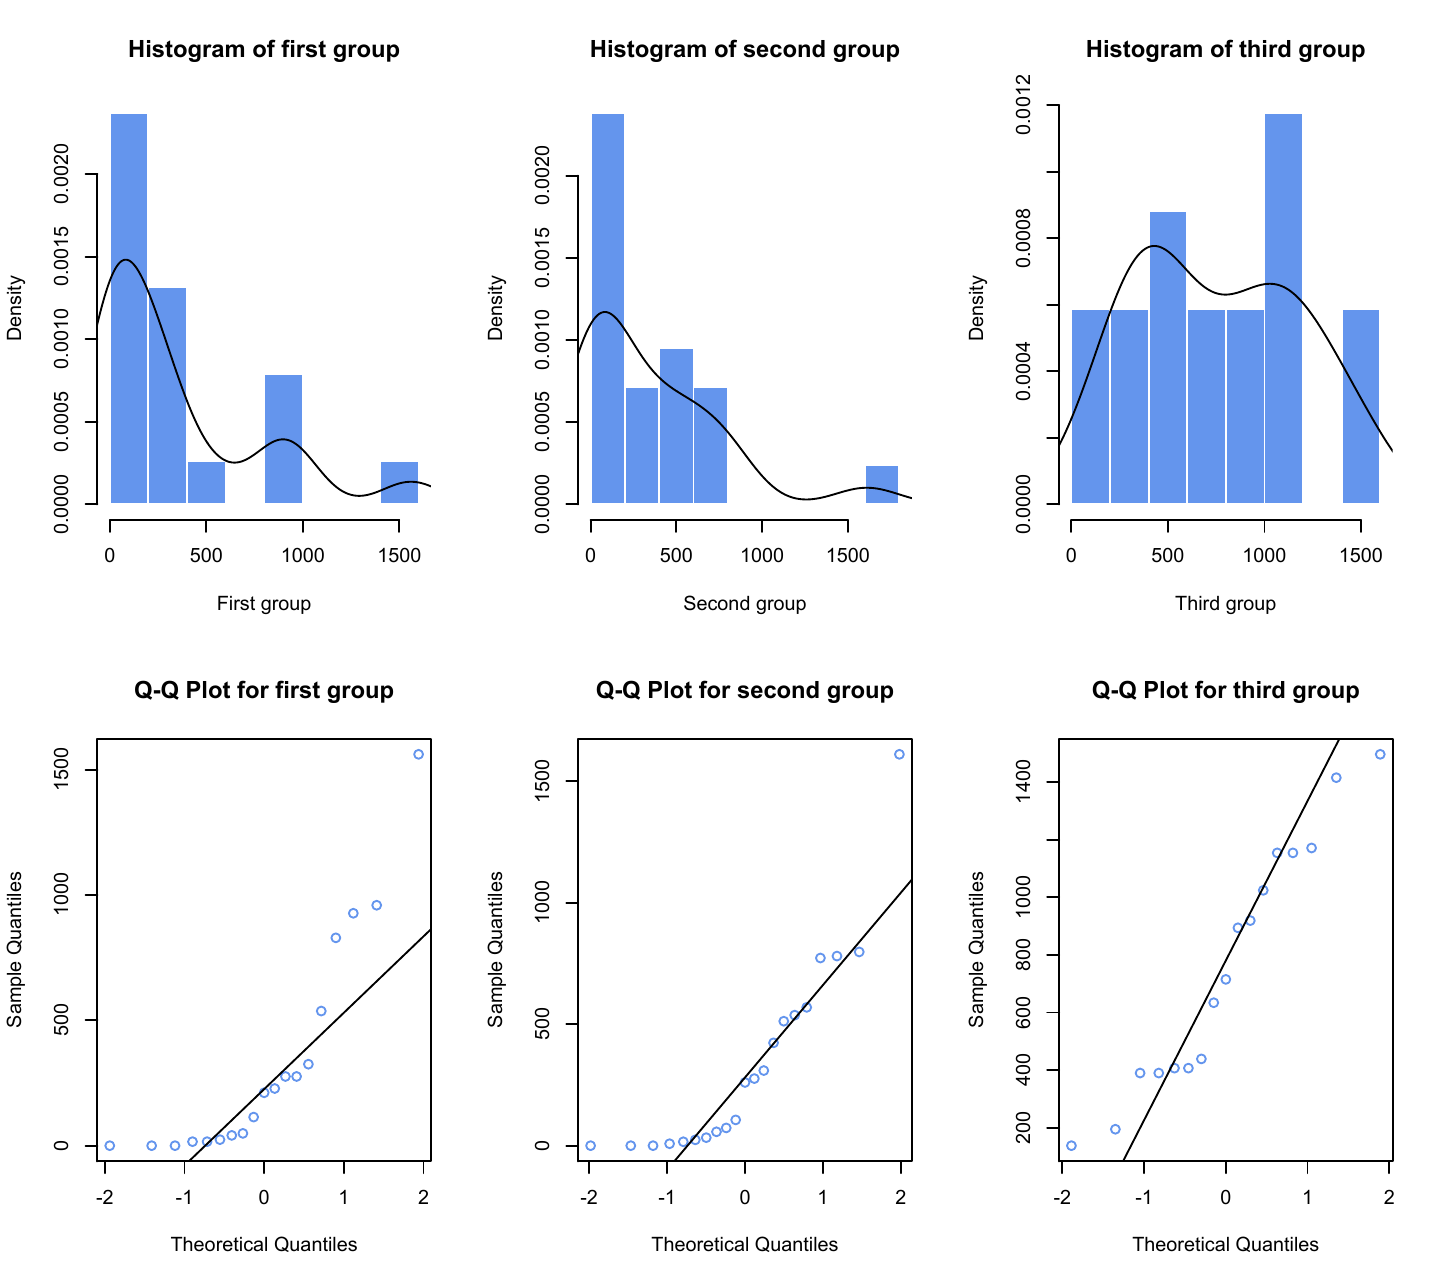
\includegraphics[width=1\textwidth]{histAlzheimer}
\caption{Model assumption checks for the \code{Amyloid} dataset using the \code{assumption.check()} function in \pkg{bayesanova}, showing that the assumption of a Gaussian mixture model is violated}
\label{fig:histAlzheimer}
\end{figure}
After loading and splitting the data into the three groups, we run the \code{assumption.check()} function:
\begin{example}
R> library(Stat2Data)
R> data(Amyloid)
R> head(Amyloid)

  Group Abeta
1   NCI   114
2   NCI    41
3   NCI   276
4   NCI     0
5   NCI    16
6   NCI   228

R> NCI = (Amyloid %>% filter(Group=="NCI"))$Abeta
R> MCI = (Amyloid %>% filter(Group=="MCI"))$Abeta
R> mAD = (Amyloid %>% filter(Group=="mAD"))$Abeta
R> assumption.check(NCI, MCI, mAD)

1: In assumption.check(NCI, MCI, mAD) :
  Model assumption of normally distributed data in each group is violated.
 All results of the Bayesian ANOVA based on a multi-component Gaussian 
 mixture could therefore be unreliable and not trustworthy.
2: In assumption.check(NCI, MCI, mAD) :
  Run further diagnostics (like Quantile-Quantile-plots) to check if the 
  Bayesian ANOVA can be expected to be robust to the violations of normality	
\end{example}
The results in  \ref{fig:histAlzheimer} clearly show that the model assumptions are violated. Therefore, it is not recommended to run a Bayesian ANOVA in this case. A solution via a traditional ANOVA or via a Bayes factor based ANOVA would not proceed at this point, too.

\subsection{A small simulation study -- Recapturing simulation parameters of synthetic datasets}
The next example is more in the veins of a simulation approach. We simulate three-, four-, five- and six-component Gaussian mixtures with increasing means $\mu_j:=j$ and $\sigma_j=1$. Therefore, the theoretical parameter values as well as the differences in means and standard deviations and the effect sizes $\delta_{lr}$ are known $\forall l,r$.
We simulate 500 datasets with $n=50$ observations in each group for each Gaussian mixture above, and run the Bayesian ANOVA with default hyperparameters, that is 10000 Gibbs steps with 5000 burn-in steps, 95\% credibility level and standard deviation output. Histograms of the posterior means for all parameters are shown in  \ref{fig:sim}.

\begin{figure}[h!]
\centering
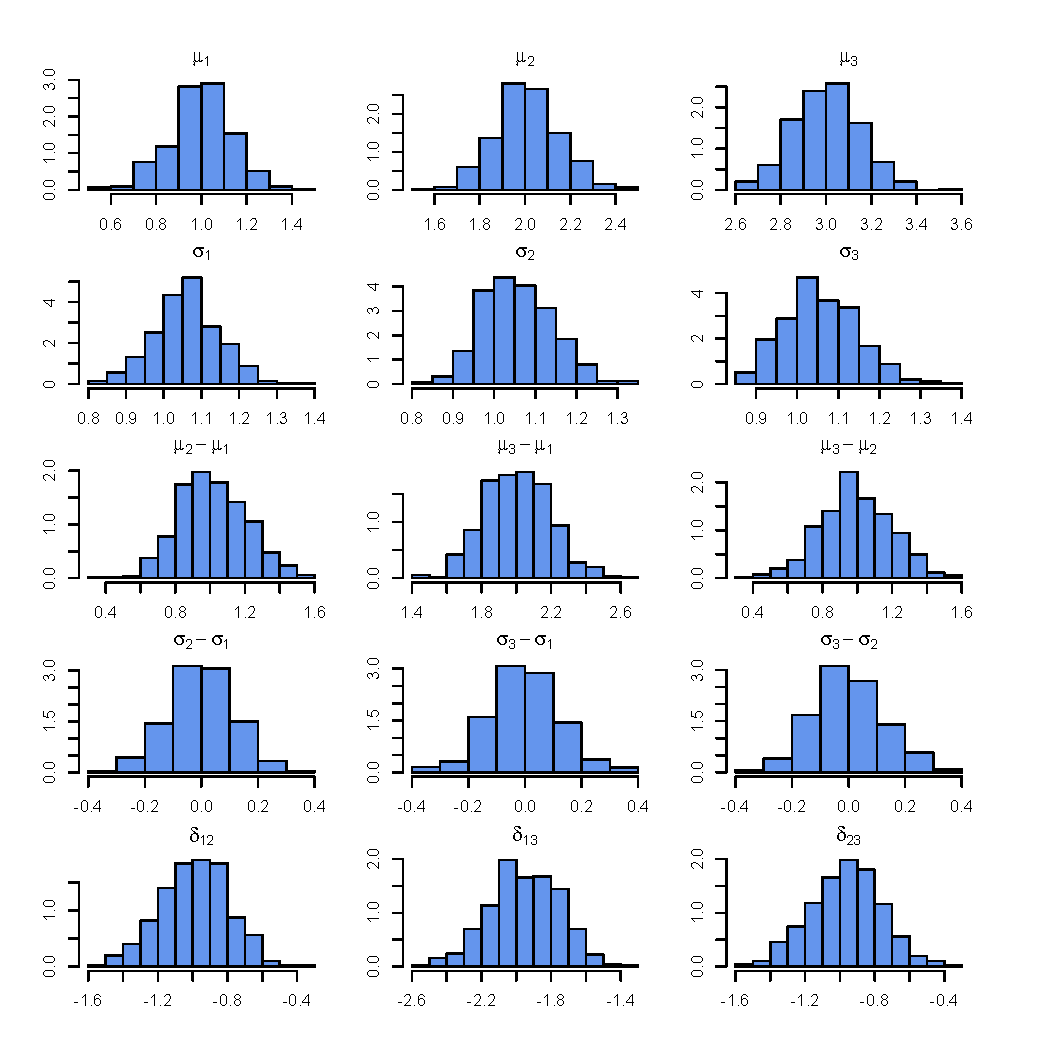
\includegraphics[width=1\textwidth]{sim}
\caption{Recapturing simulation parameters of synthetic datasets with \code{bayes.anova()}, showing that the Gibbs sampler yields consistent estimates of the underlying effect sizes}
\label{fig:sim}
\end{figure}

The results clearly show that even for $500$ simulated datasets the true parameters $\mu_j=j$ and $\sigma_j=1$ are recaptured for small sample sizes like $n=50$ in each group. Also, the differences in means $\mu_l-\mu_r, l\neq r$ are near one, and the differences in standard deviations $\sigma_l-\sigma_r, l\neq r$ are near zero. The effect sizes $\delta_{lr}, l\neq r$ also are recaptured as expected. More details about the theoretical properties of the procedure, especially the derivation of the Gibbs sampler for the two-group case can be found in \cite{Kelter2020JORSBayest,Kelter2021StatisticsInBiosciences}. Note that increasing sample sizes in the groups will yield consistent estimates as a result of MCMC theory \cite{Robert2004}.



\section{Conclusion} \label{sec:summary}
This paper introduces \pkg{bayesanova}, an R package for conducting a Bayesian analysis of variance based on MCMC in a Gaussian mixture distribution with known allocations. The Bayesian ANOVA implemented in \pkg{bayesanova} is based on Gibbs sampling and supports up to six distinct components, which covers the typical range of ANOVAs used in empirical research.

The package provides four functions to check the model assumptions, run the Bayesian ANOVA, visualize the results and check the posterior fit. All functions have a variety of optional parameters to adapt them to a specific workflow or goal. Also, convergence issues can be detected via the built-in convergence diagnostics of all MCMC results in the \code{anovaplot()} function and it is possible to post-process the results delivered as raw Markov chain draws by \code{bayes.anova}, for example via the R package \CRANpkg{bayestestR} \citep{Makowski2019a}.

In the paper, multiple examples from medical and psychological research using real datasets were provided, showing the richness of information provided by the proposed procedure. Also, while explicit testing (for example via Bayes factors) is not implemented as standard output, it is worth noting that computing Bayes factors numerically based on the Gaussian mixture model is possible for example by using numerical techniques such as the Savage-Dickey density ratio \citep{Kelter2021,Wagenmakers2010,Dickey1970,Verdinelli1995}. However, the focus of explicit hypothesis testing is replaced in the default output of the procedure by estimation of the effect sizes between groups (or component density parameters) under uncertainty. If hypothesis testing is needed, the implemented ROPE can be used for rejecting a hypothesis based on interval hypothesis tests -- compare \cite{Kelter2021BMCHodgesLehmann}, \cite{Linde2020ROPE} and \cite{Kruschke2018a} -- or by using external packages like \pkg{bayestestR} \citep{Makowski2019a} in conjunction with the raw samples provided by \code{bayes.anova}. Also, other indices like the probability of direction \citep{Makowski2019} or the MAP-based p-value \citep{Mills2018} can be obtained via the package \pkg{bayestestR} \citep{Makowski2019a} if hypothesis testing is desired, for an overview see \cite{Kelter2021}. To offer users the freedom of choice for their preferred statistical evidence measure, only a ROPE-based estimate of the maximum a posteriori effect size $\delta$ is provided in \pkg{bayesanova}.

A small simulation study showed for the case of three-component Gaussian mixtures, that the provided MCMC algorithm precisely captures the true parameter values. Similar results hold for the four- or more-component case, as can easily be checked by adapting the provided R code.

In summary, the \pkg{bayesanova} package provides a novel and easy to apply alternative to existing packages like \pkg{stats} \citep{RProgrammingLanguage} or \pkg{BayesFactor} \citep{BayesFactorPackage}, which implement the traditional frequentist ANOVA and Bayesian ANOVA models based on the Bayes factor.

Future plans include to add prior predictive checks and up to 12-component support, allowing for $2\times 6$ Bayesian ANOVAs. Also, nonparametric mixtures could be applied in the case the model assumptions are violated, but therefore first theoretical results are necessary.




\bibliography{kelter}



\address{Riko Kelter\\
  University of Siegen, Department of Mathematics\\
  Walter-Flex-Street 3\\
  57072, Siegen\\
  Germany\\
  ORCiD: 0000-0001-9068-5696\\
  \email{riko.kelter@uni-siegen.de}}
  
  
  \section*{Appendix}\label{appn}
  \subsection*{Details on the F-statistic in frequentist ANOVA}
  After observing the data, the following quantities are calculated: For group $j$, $j=1,...,k$, $I_j$ experimental units are observed and the empirical mean $m_j=1/I_j \sum_{l=1}^{I_j} y_{lj}$ and empirical variance $s_j^2=1/(I_j-1) \sum_{l=1}^{I_j} (y_{lj}-m_j)^2$ are calculated (data is assumed to be listed in a table where the groups correspond to the columns). The sum $\Sigma_{i\in I_j} y_{ij}$ and the sum of squares $\Sigma_{i\in I_j} (y_{ij})^2$ are calculated, to partition the variance into treatment and error sum of squares 
\begin{align}
	& SS_{Treatment}:=\sum_{j=1}^k I_j(m_j-m)^2 \hspace{1cm}
	SS_{Error}:=\sum_{j=1}^k (I_j-1)s_j^2 \\
	& \hspace{3cm} SS_{Total}:=\sum_{j=1}^k \sum_{i=1}^n (y_{ij}-m)^2
\end{align}
where $m:=1/k \sum_{j=1}^k m_j$. Standard calculus yields that these sums of squares can be calculated as:
\begin{align}
	& SS_{Treatment}:=\sum_{j=1}^k \frac{(\sum_i y_{ij})^2}{I_j}-\frac{(\sum_j \sum_i y_{ij})^2}{I} \hspace{1cm}
	SS_{Error}:=\sum_{j=1}^k \sum_{i}y_{ij}^2-\sum_{j}\frac{(\sum_i y_{ij})^2}{I_j} \\
	& \hspace{4cm} SS_{Total}:=\sum_{j=1}^k \sum_{i}y_{ij}^2-\frac{(\sum_j \sum_i y_{ij})^2}{I}
\end{align}
Using the corresponding degrees of freedom $DF_{Treatment}=k-1$, $DF_{Error}=n-k$ and $DF_{Total}=n-1$, the F-statistic is defined as
\begin{align}
	F=\frac{MS_{Treatment}}{MS_{Error}}	
\end{align}
where
\begin{align}
		MS_{Treatment}:=\frac{SS_{Treatment}}{DF_{Treatment}} \hspace{1cm} MS_{Error}:=\frac{SS_{Error}}{DF_{Error}}
\end{align}
using only the quantities defined above. If the F-statistic is larger than the $\alpha$-quantile for significance level $\alpha$, $H_0$ is rejected.
